%%
%% This is file `sample-sigconf-authordraft.tex',
%% generated with the docstrip utility.
%%
%% The original source files were:
%%
%% samples.dtx  (with options: `all,proceedings,bibtex,authordraft')
%% 
%% IMPORTANT NOTICE:
%% 
%% For the copyright see the source file.
%% 
%% Any modified versions of this file must be renamed
%% with new filenames distinct from sample-sigconf-authordraft.tex.
%% 
%% For distribution of the original source see the terms
%% for copying and modification in the file samples.dtx.
%% 
%% This generated file may be distributed as long as the
%% original source files, as listed above, are part of the
%% same distribution. (The sources need not necessarily be
%% in the same archive or directory.)
%%
%%
%% Commands for TeXCount
%TC:macro \cite [option:text,text]
%TC:macro \citep [option:text,text]
%TC:macro \citet [option:text,text]
%TC:envir table 0 1
%TC:envir table* 0 1
%TC:envir tabular [ignore] word
%TC:envir displaymath 0 word
%TC:envir math 0 word
%TC:envir comment 0 0
%%
%% The first command in your LaTeX source must be the \documentclass
%% command.
%%
%% For submission and review of your manuscript please change the
%% command to \documentclass[manuscript, screen, review]{acmart}.
%%
%% When submitting camera ready or to TAPS, please change the command
%% to \documentclass[sigconf]{acmart} or whichever template is required
%% for your publication.
%%
%%
\documentclass[sigconf,authordraft]{acmart}
% \documentclass[manuscript,review,anonymous]{acmart}
%%
%% \BibTeX command to typeset BibTeX logo in the docs
\AtBeginDocument{%
  \providecommand\BibTeX{{%
    Bib\TeX}}}

%% Rights management information.  This information is sent to you
%% when you complete the rights form.  These commands have SAMPLE
%% values in them; it is your responsibility as an author to replace
%% the commands and values with those provided to you when you
%% complete the rights form.
\setcopyright{acmlicensed}
\copyrightyear{2018}
\acmYear{2018}
\acmDOI{XXXXXXX.XXXXXXX}
%% These commands are for a PROCEEDINGS abstract or paper.
\acmConference[Conference acronym 'XX]{Make sure to enter the correct
  conference title from your rights confirmation email}{June 03--05,
  2018}{Woodstock, NY}
%%
%%  Uncomment \acmBooktitle if the title of the proceedings is different
%%  from ``Proceedings of ...''!
%%
%%\acmBooktitle{Woodstock '18: ACM Symposium on Neural Gaze Detection,
%%  June 03--05, 2018, Woodstock, NY}
\acmISBN{978-1-4503-XXXX-X/2018/06}


%%
%% Submission ID.
%% Use this when submitting an article to a sponsored event. You'll
%% receive a unique submission ID from the organizers
%% of the event, and this ID should be used as the parameter to this command.
%%\acmSubmissionID{123-A56-BU3}

%%
%% For managing citations, it is recommended to use bibliography
%% files in BibTeX format.
%%
%% You can then either use BibTeX with the ACM-Reference-Format style,
%% or BibLaTeX with the acmnumeric or acmauthoryear sytles, that include
%% support for advanced citation of software artefact from the
%% biblatex-software package, also separately available on CTAN.
%%
%% Look at the sample-*-biblatex.tex files for templates showcasing
%% the biblatex styles.
%%

%%
%% The majority of ACM publications use numbered citations and
%% references.  The command \citestyle{authoryear} switches to the
%% "author year" style.
%%
%% If you are preparing content for an event
%% sponsored by ACM SIGGRAPH, you must use the "author year" style of
%% citations and references.
%% Uncommenting
%% the next command will enable that style.
%%\citestyle{acmauthoryear}


%%
%% end of the preamble, start of the body of the document source.
\usepackage{booktabs,tabularx,array,subcaption,float}
\usepackage{amsmath} % For mathematical environments
\usepackage{enumitem} % For customizing lists
\usepackage{tcolorbox}
\usepackage{lipsum}
\usepackage{xcolor}

% Define a command for small italic text
\newcommand{\smallitalic}[1]{{\small\textit{#1}}}
\newcommand{\strategy}[1]{{\textit{#1}}}
\begin{document}

%%
%% The "title" command has an optional parameter,
%% allowing the author to define a "short title" to be used in page headers.
\title{Investigating Questioning Strategies for Robot Learning by Asking in Household Tasks}

%%
%% The "author" command and its associated commands are used to define
%% the authors and their affiliations.
%% Of note is the shared affiliation of the first two authors, and the
%% "authornote" and "authornotemark" commands
%% used to denote shared contribution to the research.
% \author{Ben Trovato}
% \authornote{Both authors contributed equally to this research.}
% \email{trovato@corporation.com}
% \orcid{1234-5678-9012}
% \author{G.K.M. Tobin}
% \authornotemark[1]
% \email{webmaster@marysville-ohio.com}
% \affiliation{%
%   \institution{Institute for Clarity in Documentation}
%   \city{Dublin}
%   \state{Ohio}
%   \country{USA}
% }

% \author{Lars Th{\o}rv{\"a}ld}
% \affiliation{%
%   \institution{The Th{\o}rv{\"a}ld Group}
%   \city{Hekla}
%   \country{Iceland}}
% \email{larst@affiliation.org}

% \author{Valerie B\'eranger}
% \affiliation{%
%   \institution{Inria Paris-Rocquencourt}
%   \city{Rocquencourt}
%   \country{France}
% }

% \author{Aparna Patel}
% \affiliation{%
%  \institution{Rajiv Gandhi University}
%  \city{Doimukh}
%  \state{Arunachal Pradesh}
%  \country{India}}

% \author{Huifen Chan}
% \affiliation{%
%   \institution{Tsinghua University}
%   \city{Haidian Qu}
%   \state{Beijing Shi}
%   \country{China}}

% \author{Charles Palmer}
% \affiliation{%
%   \institution{Palmer Research Laboratories}
%   \city{San Antonio}
%   \state{Texas}
%   \country{USA}}
% \email{cpalmer@prl.com}

% \author{John Smith}
% \affiliation{%
%   \institution{The Th{\o}rv{\"a}ld Group}
%   \city{Hekla}
%   \country{Iceland}}
% \email{jsmith@affiliation.org}

% \author{Julius P. Kumquat}
% \affiliation{%
%   \institution{The Kumquat Consortium}
%   \city{New York}
%   \country{USA}}
% \email{jpkumquat@consortium.net}

\author{Yuanda Hu}
\affiliation{%
  \institution{College of Design and Innovation, Tongji University}
  \city{Shanghai}
  \country{China}
}
\email{ydhu@tongji.edu.cn}

\author{Jiani Hou}
\affiliation{%
  \institution{School of Design, Southern University of Science and Technology}
  \city{Shenzhen}
  \country{China}
}

\author{Dai Shi}
\affiliation{%
  \institution{College of Design and Innovation, Tongji University}
  \city{Shanghai}
  \country{China}
}

\author{Suming Li}
\affiliation{%
  \institution{College of Architecture and Urban Planning, Tongji University}
  \city{Shanghai}
  \country{China}
}
\email{SunnyMing@tongji.edu.cn}

\author{Yujie Qiu}
\affiliation{%
  \institution{School of Mechanical and Manufacturing Engineering, University of New South Wales}
  \city{Sydney}
  \state{NSW}
  \country{Australia}
}
\email{z5637231@ad.unsw.edu.au}

\author{Yate Ge}
\affiliation{%
  \institution{College of Design and Innovation, Tongji University}
  \city{Shanghai}
  \country{China}
}
\email{geyate@tongji.edu.cn}

\author{Qi Wang}
\affiliation{%
  \institution{College of Design and Innovation, Tongji University}
  \city{Shanghai}
  \country{China}
}

\author{Xiaohua Sun}
\affiliation{%
  \institution{School of Design, Southern University of Science and Technology}
  \city{Shenzhen}
  \state{Guangdong}
  \country{China}
}

\author{Weiwei Guo}
\affiliation{%
  \institution{College of Design and Innovation, Tongji University}
  \city{Shanghai}
  \country{China}
}


%%
%% By default, the full list of authors will be used in the page
%% headers. Often, this list is too long, and will overlap
%% other information printed in the page headers. This command allows
%% the author to define a more concise list
%% of authors' names for this purpose.
\renewcommand{\shortauthors}{Trovato et al.}

%%
%% The abstract is a short summary of the work to be presented in the
%% article.
\begin{abstract}
How can robots learn to complete complex household tasks that involve diverse preferences and exceptions? We investigate how different questioning strategies shape robot learning in interactive settings. From a formative human–human study, we identified three strategies: User-Preference-First, Parallel Exploration, and Direct Querying. We implemented them in a multi-modal LLM-based questioning framework, where prompt manipulation enables flexible configuration of strategies. Deploying the framework on a humanoid robot, we conducted a user study (N=18) across three tidying scenarios. Results show that participants naturally exhibited three questioning patterns in household teaching—Direct Querying, Parallel Exploration, and User-Preference-First. These patterns were successfully instantiated as controllable strategies on a robot, producing consistent and comparable multi-turn behaviors. In a user study ($N=18$), the strategies led to significant differences in workload, self-efficacy, and related user perceptions.
\end{abstract}

%%
%% The code below is generated by the tool at http://dl.acm.org/ccs.cfm.
%% Please copy and paste the code instead of the example below.
% %%
% \begin{CCSXML}

% <ccs2012>
%  <concept>
%   <concept_id>00000000.0000000.0000000</concept_id>
%   <concept_desc>Do Not Use This Code, Generate the Correct Terms for Your Paper</concept_desc>
%   <concept_significance>500</concept_significance>
%  </concept>
%  <concept>
%   <concept_id>00000000.00000000.00000000</concept_id>
%   <concept_desc>Do Not Use This Code, Generate the Correct Terms for Your Paper</concept_desc>
%   <concept_significance>300</concept_significance>
%  </concept>
%  <concept>
%   <concept_id>00000000.00000000.00000000</concept_id>
%   <concept_desc>Do Not Use This Code, Generate the Correct Terms for Your Paper</concept_desc>
%   <concept_significance>100</concept_significance>
%  </concept>
%  <concept>
%   <concept_id>00000000.00000000.00000000</concept_id>
%   <concept_desc>Do Not Use This Code, Generate the Correct Terms for Your Paper</concept_desc>
%   <concept_significance>100</concept_significance>
%  </concept>
% </ccs2012>
% \end{CCSXML}

\begin{CCSXML}
<ccs2012>
   <concept>
       <concept_id>10003120.10003121</concept_id>
       <concept_desc>Human-centered computing~Human computer interaction (HCI)</concept_desc>
       <concept_significance>500</concept_significance>
       </concept>
   <concept>
       <concept_id>10010147.10010178.10010199.10010204</concept_id>
       <concept_desc>Computing methodologies~Robotic planning</concept_desc>
       <concept_significance>300</concept_significance>
       </concept>
   <concept>
       <concept_id>10010147.10010178.10010179.10010181</concept_id>
       <concept_desc>Computing methodologies~Discourse, dialogue and pragmatics</concept_desc>
       <concept_significance>300</concept_significance>
       </concept>
 </ccs2012>
\end{CCSXML}

\ccsdesc[500]{Human-centered computing~Human computer interaction (HCI)}
\ccsdesc[300]{Computing methodologies~Robotic planning}
\ccsdesc[300]{Computing methodologies~Discourse, dialogue and pragmatics}
\ccsdesc[500]{Human-centered computing~Empirical studies in HCI}

% \ccsdesc[500]{Do Not Use This Code~Generate the Correct Terms for Your Paper}
% \ccsdesc[300]{Do Not Use This Code~Generate the Correct Terms for Your Paper}
% \ccsdesc{Do Not Use This Code~Generate the Correct Terms for Your Paper}
% \ccsdesc[100]{Do Not Use This Code~Generate the Correct Terms for Your Paper}

%%
%% Keywords. The author(s) should pick words that accurately describe
%% the work being presented. Separate the keywords with commas.
% \keywords{Do, Not, Us, This, Code, Put, the, Correct, Terms, for,
%   Your, Paper}
\keywords{Human-Robot Interaction, Questioning Strategies, Vision-Language Models, User Study}

%% A "teaser" image appears between the author and affiliation
%% information and the body of the document, and typically spans the
%% page.
\begin{teaserfigure}
  
\includegraphics[width=\textwidth]{teaser}
  \caption{We study how robots can learn household tasks through questioning. Our work (1) identifies distinct questioning patterns in human teaching, (2) instantiates them as three modular strategies—\textit{Direct Querying}, \textit{Parallel Exploration}, and \textit{User-Preference-First}—on a humanoid robot, and (3) evaluates their effects on user perception, interaction, and experience in personalized task learning.}
  \Description{Enjoying the baseball game from the third-base
  seats. Ichiro Suzuki preparing to bat.}
  \label{fig:teaser}
\end{teaserfigure}

\received{20 February 2007}
\received[revised]{12 March 2009}
\received[accepted]{5 June 2009}

%%
%% This command processes the author and affiliation and title
%% information and builds the first part of the formatted document.
\maketitle

\section{Introduction}
Household tasks are inherently open-ended and shaped by diverse user preferences, making it difficult for robots to reliably align with human expectations \cite{wu2023tidybot,nasiriany2024robocasa}. Beyond perceiving the physical environment, effective assistance requires robots to proactively acquire and adapt to individual preferences \cite{zheng2019personalized,lawley2024val}. Learning by Asking (LBA) provides a natural and efficient mechanism to reduce uncertainty, clarify intentions, and gradually build common ground with users \cite{biyik2019asking,6padmakumar2022teach,8leusmann2025investigating}. For example, in an organizing task, a robot might ask about each object in turn, such as ``Should this book go on the shelf?'' or ``Should this pen stay on the desk?'', or instead begin with a more general question such as ``Do you usually separate study materials from daily supplies?''. Prior work in human teaching and collaboration shows that questioning strongly shapes communication efficiency and perceived control \cite{cakmak2012designing,mutlu2009footing}. We thus infer that  household human-robot interaction is also necessary to flexibly employ multiple questioning strategies.


A substantial body of work has examined active question-asking in robotics as a computational mechanism to sample uncertain data and reduce task ambiguity \cite{cakmak2012designing,biyik2019asking,habibian2022here}. Yet, such approaches overlook a fundamental issue: in household teaching scenarios, what distinct questioning patterns do humans naturally exhibit, and how might these patterns be abstracted and transferred into robot interaction? Although prior work has examined predefined or rule-based questioning in HRI to support teaching and engagement \cite{12biyik2019asking}, systematic investigation remains limited \cite{robinson2023probing,hu2024designing} and these approaches do not capture the diversity of questioning strategies observed in real instructional contexts. Rule-based systems have limited flexibility in open-ended settings, which constrains their use for systematic comparison of questioning strategies. Recent advances in large language models (LLMs) and vision--language models (VLMs) enable the generation of multi-turn, context-sensitive dialogue and allow prompt design to configure different questioning styles, supporting the evaluation of human-identified patterns in robotic interaction \cite{driess2023palm,huang2023instruct2act,8leusmann2025investigating}.


We begin with a preliminary question: in household teaching of personalized tasks, do humans naturally exhibit distinguishable questioning patterns (RQ1)? To answer this, we conducted a formative human--human study and identified three candidate patterns that describe how people acquire information and express preferences during task instruction. Based on these findings, large language models (LLMs) and vision--language models (VLMs) allow us to implement these patterns as controllable questioning strategies and to support multi-turn, context-sensitive interaction. This raises our second research question: can these human-derived patterns be deployed as stable and controllable ``questioning strategies'' on robots and produce consistent behaviors in real interaction (RQ2)? To address this, we designed a modular VLM-based framework that enables robots to generate questions in a controlled way across multiple turns and to use user answers for preference learning and task execution. Finally, we conducted a user study in household tidying scenarios ($N=18$) to compare different strategies in terms of workload, self-efficacy, and related user perceptions, thereby addressing RQ3.


Our results show that participants naturally exhibited three distinguishable questioning patterns—Direct Querying (item-by-item questions), Parallel Exploration (interleaving preference and action queries), and User-Preference-First (eliciting general rules before specific actions)—confirming our hypothesis about the existence of such patterns (RQ1).On the robot side, these patterns were successfully deployed as controllable questioning strategies (RQ2) and produced consistent and comparable behaviors in multi-turn interaction. In the user study ($N=18$), we further found significant differences across strategies (RQ3), including perceived efficiency, sense of control, subjective workload, and objective measures such as number of turns and task completion time. This work establishes a foundation for systematically introducing and comparing questioning strategies in household human--robot collaboration, and demonstrates how human-derived questioning patterns can be translated into controllable robot behaviors with a reproducible framework. Our key contributions are:
\begin{enumerate}
  \item Identifying and empirically validating three distinct questioning patterns in household teaching scenarios;
  \item Designing and implementing a configurable VLM-based framework that deploys these strategies under comparable task capabilities;
  \item Providing empirical evidence on how different strategies affect user perceptions and outcomes in long-horizon household tasks.
\end{enumerate}


\section{Related Work}
\subsection{Robot Learning in Household Tasks}

In household tasks, successful robot performance often hinges on capturing deeper information that reflects user characteristics and contextual variations, which cannot be fully encoded in advance \cite{zhong2021gap}. To address this, researchers have explored learning approaches that acquire user preferences or constraints through dynamic human–robot interaction. Based on who initiates the exchange, existing work can be divided into three categories: human-initiated teaching, interactive learning, and robot-initiated learning.

Human-initiated teaching transfers task knowledge or preferences through demonstrations or explicit instructions, focusing on extracting useful information from user input. Examples include trajectory imitation for complex operations \cite{tsuji2025survey,hussein2017imitation,wake2024gpt}  or combining language with demonstrations to teach new skills \cite{she2014teaching}. To support such methods, the research community has developed large-scale simulation platforms and multi-modal datasets—for example, RoboCasa \cite{nasiriany2024robocasa} offers a scalable environment for everyday task simulation, while the NatSGD dataset provides speech, gesture, and demonstration data to facilitate learning in natural human–robot interaction scenarios \cite{shrestha2024natsgd}.

Interactive learning emphasizes bidirectional exchange, where robots and users iteratively build task understanding through dialogue, corrections, and demonstrations. Methods such as Interactive Task Learning  and dialogue-based lifelong learning explore how to incrementally integrate new information while retaining prior knowledge \cite{tyshka2023interactive,reimann2024survey,schmidt2018survey,luo2019learning,zheng2019personalized,lawley2024val} .

Robot-initiated learning reduces uncertainty by actively posing questions or probing. A typical method is active learning, which centers on selecting the most valuable questions based on uncertainty or utility functions, while balancing information gain against the burden placed on the human respondent. For example, some studies propose questioning strategies that both reveal the current knowledge of the robot and remain easy for humans to interpret \cite{habibian2022here}, as well as user-friendly active querying methods that are easy to answer\cite{biyik2019asking}. Other approaches attempt to learn from observing user actions and feedback \cite{wu2023tidybot}. However, when relying solely on robot-driven learning without user involvement, these methods remain insufficient to fully capture the deeper-level information required for task completion.

Overall, each approach has distinct strengths: human teaching depends on high-quality demonstrations, interactive learning builds on long-term accumulation, and robot-initiated learning emphasizes efficient exploration. For long-duration household tasks such as organizing refrigerators or arranging objects, multi-turn robot questioning offers a natural and effective way to uncover deeper information \cite{hunt2024survey}. Therefore, we focuses on the study and application of multi-turn active questioning strategies in household settings.

\subsection{Learning By Asking in Human–Robot Interaction}
In human robot interaction research, learning by asking has been emerging as an important approach to endowing robots with intelligent behaviors. Its core idea is to enable robots to actively acquire information by posing questions~\cite{hu2025task,shen2025elba}.Existing active learning strategies can be broadly categorized into three types: 
(i) ambiguity-resolution questioning, where robots ask specific questions (e.g., ``Which cup?'' or ``Where exactly is `next to'?'' ) to clarify referential or semantic ambiguities in instructions~\cite{3ren2023robots,4andukuri2024star,5ramrakhya2025grounding,6padmakumar2022teach}; 
(ii) knowledge-completion questioning, where robots seek missing information during task planning (e.g., ``I don't know what is inside this drawer'')~\cite{hu2025task,7uehara2024learning}; 
and (iii) curiosity-driven exploratory questioning, where robots investigate unknown objects or areas to expand their knowledge base~\cite{8leusmann2025investigating,9carter2022you,10leusmann2025developing,11scialom2019ask}.

However, these methods typically target relatively simple task settings~\cite{7uehara2024learning,12biyik2019asking,13gonzalez2018analyzing}, such as evaluating whether a single clarification resolves ambiguity~\cite{5ramrakhya2025grounding,7uehara2024learning} or asking once to acquire knowledge about a novel object~\cite{12biyik2019asking,shen2019learning}. While such atomic questioning strategies are effective in isolated cases, naively extending them to long-horizon tasks often results in unstructured questioning, which can degrade user experience, reduce interaction efficiency, and create a mechanical impression. This highlights the need for macro-level planning in human--robot question--answering~\cite{oviatt2006human,kosch2023survey,tyshka2023interactive}. The underlying limitation lies in an emphasis on how to ask (e.g., algorithmic follow-ups) while neglecting when, in what order, and for what purpose to ask~\cite{tyshka2023interactive,hu2024designing}. Studies on cognitive load further show that frequent attentional shifts can impair cognitive performance~\cite{kosch2023survey}.

By contrast, the dialogue systems community has demonstrated that strategic questioning is key to managing multi-turn tasks, as it reduces cognitive burden and improves efficiency~\cite{stivers2010overview,kwan2023survey}. For instance, Stivers' analysis shows that macro-level planning of polar and wh-question sequences (e.g., prioritizing confirmations) optimizes information gathering~\cite{stivers2010overview}, while reinforcement learning approaches in dialogue rely on policies to handle long sequences~\cite{kwan2023survey}.

In summary, while strategy-driven questioning has been shown to enhance coherence and effectiveness in multi-turn dialogue systems, HRI research has largely focused on optimizing individual questions, with limited attention to macro-level organization in long-horizon tasks~\cite{hu2024designing}. This paper therefore focuses on household scenarios involving long-duration tasks, aiming to understand how user experience and interaction efficiency are affected when robots strategically plan their questions while actively acquiring user preferences.




\subsection{Dialogue and Questioning Strategies}
Research on questioning in dialogue can generally be divided into two categories: theoretical studies and applied explorations in human–robot interaction. The former provide a methodological foundation for understanding how to ask, while the latter demonstrate how these methods can be implemented in practical systems.

Theoretical studies mainly based on education and qualitative research methodology. Educational research emphasizes the relationship between cognitive levels of questioning and learning outcomes, examining how teachers design questions to foster deeper thinking and self-monitoring in students~\cite{redfield1981meta,tofade2013best}. Empirical evidence and teaching practices further suggest that strategies such as waiting time, follow-up questioning, and self-questioning training play an important role in classroom effectiveness~\cite{redfield1981meta,tofade2013best}. Qualitative research has developed a set of operational tools to support probing for deeper information ~\cite{robinson2023probing,balza2022effective,dejonckheere2019semistructured}. For example, probing studies identify different types of follow-up questions and highlight their role in building trust, avoiding bias, and ensuring data credibility~\cite{robinson2023probing}; while semi-structured interviewing distills key skills for designing and conducting follow-up questions in research practice~\cite{dejonckheere2019semistructured}. Together, these theoretical and methodological contributions provide important insights for the design of questioning strategies in HRI.

In HRI research, some studies have directly drawn on these theories to design questioning mechanisms for dialogue agents or robots~\cite{hu2024designing,cakmak2012designing,habibian2022here}. Other work explores the generation of human-like questions under uncertainty~\cite{shin2023uncertainty} and the use of questioning strategies to improve information gathering~\cite{hu2025task}. A further line of research frames questioning as an interaction strategy that balances task efficiency with human workload. Typical scenarios include gradually acquiring knowledge through interaction with humans.\cite{adamson2021we} or requesting expert assistance at appropriate times during embodied tasks \cite{singh2022ask4help}. These studies model questioning as a decision-making problem, aiming to balance task performance with the quality of human–robot collaboration.

Despite these advances, limitations remain when applying such methods to multi-turn questioning in real-world HRI scenarios. In particular, for long-duration household tasks, there is still little guidance on how robots might employ more natural questioning strategies to acquire and update user preferences, thereby uncovering deeper-level information. To address this gap, this paper observes human face-to-face teaching in domestic settings, identifies natural questioning patterns, and maps them onto robot-specific questioning strategies for HRI.

\subsection{VLM for Robotics}
With the rapid development of vision–language models (VLMs) and large language models (LLMs), robots have made significant progress in perception, reasoning, and task execution in open environments. Representative works such as PaLM-E~\cite{driess2023palm} and RT-2~\cite{zitkovich2023rt} demonstrate that VLMs can unify multimodal perception and language reasoning, exhibiting cross-modal transfer and semantic generalization in complex tasks. Related surveys~\cite{ma2024survey,zeng2023large} further highlight VLMs/LLMs as a key technological foundation for natural interaction and long-horizon planning in embodied intelligence.

However, existing research often treats VLMs as black-box generators directly applied to instruction parsing or action planning. For example, Instruct2Act~\cite{huang2023instruct2act} and Manual2Skill~\cite{tie2025manual2skill} showcase the effectiveness of VLMs in understanding complex instructions and executing long-horizon tasks, but do not provide controllable design or systematic study of questioning strategies. Some efforts have explored asking for help under uncertainty~\cite{3ren2023robots,5ramrakhya2025grounding} or leveraging questions to improve performance in specific tasks~\cite{4andukuri2024star,shen2025elba}, yet these remain limited to isolated scenarios and lack a controllable, systematic approach to questioning.

In contrast, this work does not simply treat VLMs as black boxes. Instead, we propose a configurable VLM-based framework for questioning. The goal of this framework is not to directly realize questioning strategies in dialogue, but to provide a platform for controllable guidance of questioning patterns and for comparative experiments, thereby offering a basis for future research on questioning strategies.


\section{Human–Human Study of Questioning Patterns}
Previous research has highlighted the critical role of questioning in aligning user preferences and facilitating collaboration~\cite{cakmak2012designing,hu2024designing}. However, it remains unclear whether people employ systematic patterns of questioning when performing such tasks. For example, a learner might directly ask for overarching preferences at the outset, or alternatively, infer and confirm preferences incrementally based on contextual cues. To investigate this, we conducted a \textit{Human--Human Interaction (HHI) study} focusing on representative household tasks. In each session, one participant acted as the ``teacher,'' responding according to their personal habits and preferences, while the other participant played the role of the ``learner,'' who could only acquire task-relevant knowledge by asking questions. By analyzing these dialogues, our goal was to uncover whether the sequences of questions exhibited recognizable structures, and if so, how these structures manifested as distinct patterns across different stages of the task---namely, eliciting preferences, guiding operational steps, and accomplishing the final goal.

\subsection{Participants}
We first recruited participants through a screening questionnaire, which asked them to report the number of times they had completed the tasks of ``organizing a refrigerator'' and ``mixing cocktails'' in the past ten months, as well as to provide basic demographic information and self-rated task familiarity. We collected 34 valid responses and subsequently expanded the recruitment, resulting in a total of 40 volunteers from a university community. All participants received monetary compensation. 

Based on the questionnaire results, participants who had performed a given task more than three times in the past ten months were classified as \textit{task-familiar}, while those who had performed it once or fewer times were classified as \textit{task-unfamiliar}. In the experimental design, task-familiar participants were assigned the role of \textit{teacher}, responsible for answering questions according to their own habits and preferences. Task-unfamiliar participants were assigned the role of \textit{learner}, who could only acquire task-relevant information by asking questions. To ensure balanced comparisons, we adopted a pairing strategy, randomly assigning each teacher to a learner. In total, 14 dyads (28 participants) were invited to take part in the formal experiment. 

Participants had a mean age of 22 years and were either undergraduate or graduate students with normal or corrected-to-normal vision. All participants provided informed consent prior to the study. Teachers were instructed to familiarize themselves with the experimental environment and to imagine it as part of their everyday household setting, so as to naturally reproduce their authentic operational habits and preferences.


\subsection{Procedure}
We selected two representative household tasks for this study: organizing a refrigerator and mixing cocktails. Following prior work~\cite{dai2024think}~\cite{racca2018active}, household service tasks can generally be divided into two categories: (1) tasks that primarily aim to achieve a final desired state, such as organizing storage spaces or arranging items, and (2) tasks that emphasize procedural steps and order, such as cooking or cocktail preparation. The refrigerator organization task centers on achieving a coherent and efficient arrangement of items, while the order of specific steps is relatively flexible. In contrast, cocktail mixing requires sequential completion of subtasks with fixed ratios and procedures. By selecting these two tasks, we aimed to capture questioning strategies across different task structures. 

In the experiment, participants were paired to complete the tasks collaboratively. The \textit{learner} could only obtain information through asking questions and had to execute the physical operations accordingly. The \textit{teacher}, in turn, answered questions based on their own habits and preferences but did not perform any physical actions. We emphasized that teachers should rely solely on the verbal modality, without using demonstration-based teaching or collaborative manipulation. Thus, learners were required to depend entirely on questioning to gradually infer the teacher’s rules or preferences and proceed with the task. 

Before the main trials, teachers were instructed to familiarize themselves with the experimental environment and to imagine it as part of their everyday household setting, enabling them to reproduce their authentic habits naturally. Each pair of participants then completed two tasks in sequence: first organizing the refrigerator, followed by mixing cocktails. The completion of each task was determined by the participants themselves, who informed the experimenter once they considered the task finished. To ensure comprehensive analysis, we recorded the entire process with a GoPro Hero 9 camera, capturing both audio and video of the participants’ questioning, responses, and task operations. Figure~\ref{fig:procedure} illustrates two example interactions from the experiment.

\begin{figure}[t]
  \centering
  \includegraphics[width=\linewidth]{img/3.2.png}
  \caption{Illustration of the experimental procedure. 
  Left: In the refrigerator organization task, the learner asks about the teacher’s organizing principles (e.g., ``Do you organize by beverage type or by box height?''). 
  Right: In the cocktail mixing task, the learner queries the teacher’s preferences (e.g., ``Do you like fruit-based drinks?'').}
  \label{fig:procedure}
\end{figure}

\subsection{Hierarchical Coding Framework}
To systematically analyze how humans ask questions in task-oriented dialogues, we developed a hierarchical coding framework with three levels. At the first level, each question is annotated by its \textit{knowledge type} (Knowledge-level Annotation). At the second level, questions are further coded according to their \textit{interactional intent} (Intent-level Coding). At the third level, sequences of questions are analyzed to identify recurring \textit{patterns} across dialogues (Pattern Identification). Figure~\ref{fig:annotation-pipeline} illustrates this process, showing how raw dialogues are progressively annotated and abstracted to yield the questioning patterns.

\begin{figure}[t]
  \centering
  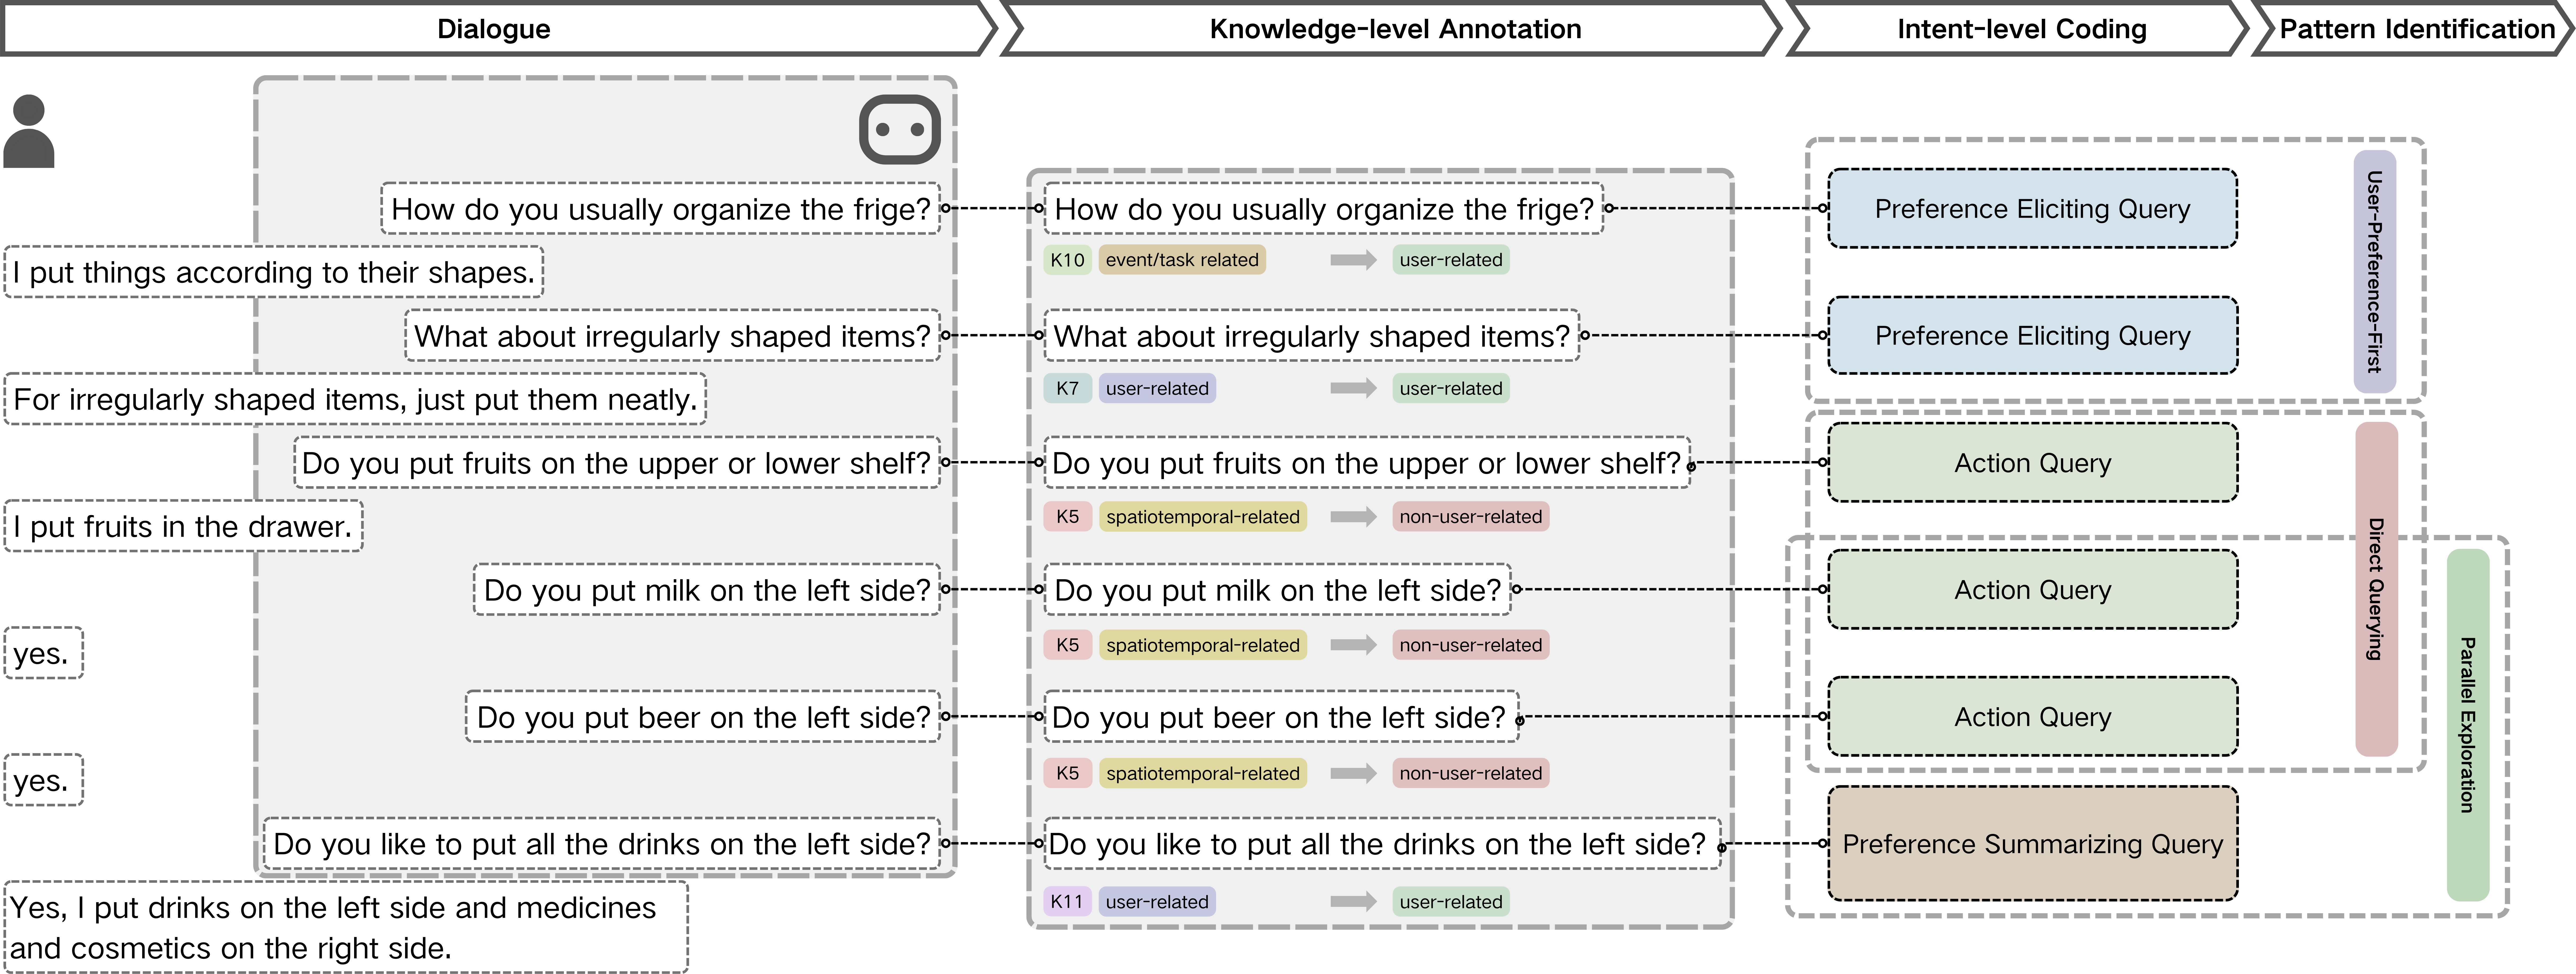
\includegraphics[width=\linewidth]{img/3.3.png}
  \caption{An illustration of the annotation pipeline: starting from raw human–robot dialogues, each question is first labeled by knowledge type, then coded for interactional intent, and finally abstracted into higher-level questioning patterns. This hierarchical process bridges low-level utterances and dialogue-level strategies.}
  \label{fig:annotation-pipeline}
\end{figure}

\subsubsection{Knowledge-level Annotation}
At the most fundamental level, we annotated each question with its corresponding knowledge type. To this end, we combined the K-type framework~\cite{shin2023uncertainty} with Wilson’s model of information behavior~\cite{wilson1999models}, allowing us to capture both the knowledge content of the question and whether it reflects user preferences. 

The K-type framework originates from cognitive psychology and educational research~\cite{redfield1981meta}~\cite{tofade2013best}, and enables a fine-grained categorization of questions according to the type of knowledge being solicited. It contains 11 categories ranging from objective factual knowledge (e.g., object identity, quantity, spatial location) to more complex subjective information (e.g., intentions, preferences, mental states). For example:
\begin{itemize}
    \item ``Is this a face mask?'' $\rightarrow$ Object Identity (K1);
    \item ``Should all the unopened stuff go on this shelf?'' $\rightarrow$ Spatial Layout (K5);
    \item ``Which part should we organize next?'' $\rightarrow$ Procedure (K8);
    \item ``Do you usually keep all the drinks on the door?'' $\rightarrow$ Internal State (K11).
\end{itemize}

We assume that the knowledge type of a question partly reflects the asker’s cognitive intent, as the focus of a question during task execution can indicate the asker’s immediate goals. The full K-type categories are presented in the Appendix (Table~\ref{tab:k-type}). 

However, while the K-type framework provides detailed knowledge classification, it does not explicitly account for task context or user preferences. For instance, the question ``Do you want the juice on the bottom or the top?'' would be classified as Spatial Layout (K5) under K-type, yet its core function is to \textit{elicit the user’s preference}, which K-type alone cannot capture. 

To address this limitation, we incorporated Wilson’s information behavior model as a complementary dimension. This model classifies questions according to information focus and task context, such as Object-related, Spatiotemporal-related, Event/Task-related, and User-related. In this study, we place particular emphasis on user preferences, and therefore we simplified the coding into two categories: \textbf{User-related}: Questions concerning user preferences, habits, or decisions; \textbf{Non-user-related}: Questions that do not involve user preferences.


In summary, each question was assigned two labels: (1) its knowledge type according to the K-type framework, and (2) whether it was user-related or non-user-related according to Wilson’s model. Figure~\ref{fig:annotation-pipeline} illustrates the distribution of several sample questions under this dual classification scheme. As shown, while multiple questions may share the same K-type category (e.g., Spatial Layout K5 or Procedure K8), Wilson’s complementary dimension allows us to further distinguish those that involve user preferences, thereby revealing the functional differences of questions within the interaction process more clearly.

\subsubsection{Intent-level Coding}
Annotating knowledge type alone is insufficient to reveal the actual function of a question in dialogue. Even when two questions share the same knowledge type, they may serve very different purposes in interaction. To capture these differences, we conducted a higher-level coding of each question based on its \textit{intent}, identifying what the asker aimed to achieve in a given context. 

Through iterative comparison and discussion, we distilled three stable categories of interactional intent, each with clear coding criteria:  \textbf{Action-oriented queries}. These questions focus on the concrete execution of the task and aim to clarify “how to do” something. If a question concerns the properties of an object, spatial arrangement, or procedural steps without involving user preferences, we coded it as action-oriented. For example, \textit{``Should this notebook be placed in the drawer?''} directly advances task execution. \textbf{Preference-summarizing queries}. As dialogues progress, questions often shift toward integrating and confirming previously gathered information. Such questions typically take a summarizing or hypothetical tone, inviting the user to confirm or correct. Questions beginning with phrases like \textit{``So\ldots''} or \textit{``Is it correct that\ldots''}
and drawing inferences from earlier answers were coded as preference-summarizing. For instance, \textit{``So you prefer to keep drinks on the upper shelf, right?''} represents this type. \textbf{Preference-eliciting queries}. These questions usually occur in the early or middle stages of a task and aim to gather the user’s overall tendencies or preferences at a choice point. The criterion here is whether the question explicitly prompts the user to select among multiple possible options. A typical example is \textit{``Do you want fruits placed above or below the drinks?''}. Such questions help the learner gradually build an understanding of the teacher’s habits.


By coding questions at the level of intent, we transform static knowledge annotations into dynamic representations of interactional goals, thereby uncovering the functional role of questions in task collaboration.


\subsubsection{Pattern Identification}
After completing intent-level coding for individual questions, we further treated the entire dialogue sequence as the unit of analysis to identify recurring questioning patterns. To achieve this, we analyzed the temporal distribution of different question types according to the coding rules described above. Two researchers independently annotated and classified 28 dialogue sequences, and any disagreements were resolved through discussion. Ultimately, we summarized three stable and representative questioning patterns (see Table~\ref{tab:patterns}). 

\begin{itemize}
    \item \textbf{User-Preference-First}. In this pattern, participants typically begin the dialogue by directly asking about the user’s personal habits or preferences, which then serve as the basis for subsequent decisions. The criterion is that if the first question in the sequence is classified as a preference-eliciting query and is followed mainly by action-oriented queries, the sequence is coded as User-Preference-First. This reflects a \textit{top-down} reasoning pathway: establishing global high-level rules first, then mapping them onto concrete operations. For example, the learner may begin with \textit{“Do you prefer to keep drinks on the door or inside the fridge?”} before proceeding with action-oriented questions such as \textit{“Should this milk be placed on the upper shelf?”}.
    
    \item \textbf{Parallel Exploration}. In this pattern, participants interleave action-oriented questions with preference-related ones throughout the task, thereby continuously integrating user preferences while advancing operations. The criterion is that preference-eliciting or preference-summarizing questions appear not only at the beginning but also in the middle or later stages of the sequence. This reflects a \textit{bottom-up} reasoning pathway: accumulating evidence through action-oriented queries and gradually extracting or validating high-level preferences, resulting in a “do-and-induce” loop. For example, while placing items, the learner may intermittently ask \textit{“Does this arrangement match your usual habit?”}.
    
    \item \textbf{Direct Querying}. Unlike the other two patterns, this type of dialogue is entirely focused on action-oriented questions, with little or no attempt to elicit or summarize user preferences. The criterion is that the entire sequence consists solely of action-oriented queries, without preference-eliciting or preference-summarizing ones. This reflects a single-layer, reactive logic in which the learner behaves more like an executor of instructions than an interpreter of user preferences.
\end{itemize}

In summary, these three patterns reveal different organizational logics of multi-turn questioning: User-Preference-First emphasizes top-down reasoning, Parallel Exploration emphasizes iterative alternation between low- and high-level reasoning, while Direct Querying remains at the level of immediate operations, as shown in 
Figure~\ref{fig:annotation-framework}.

\begin{figure}[t]
  \centering
  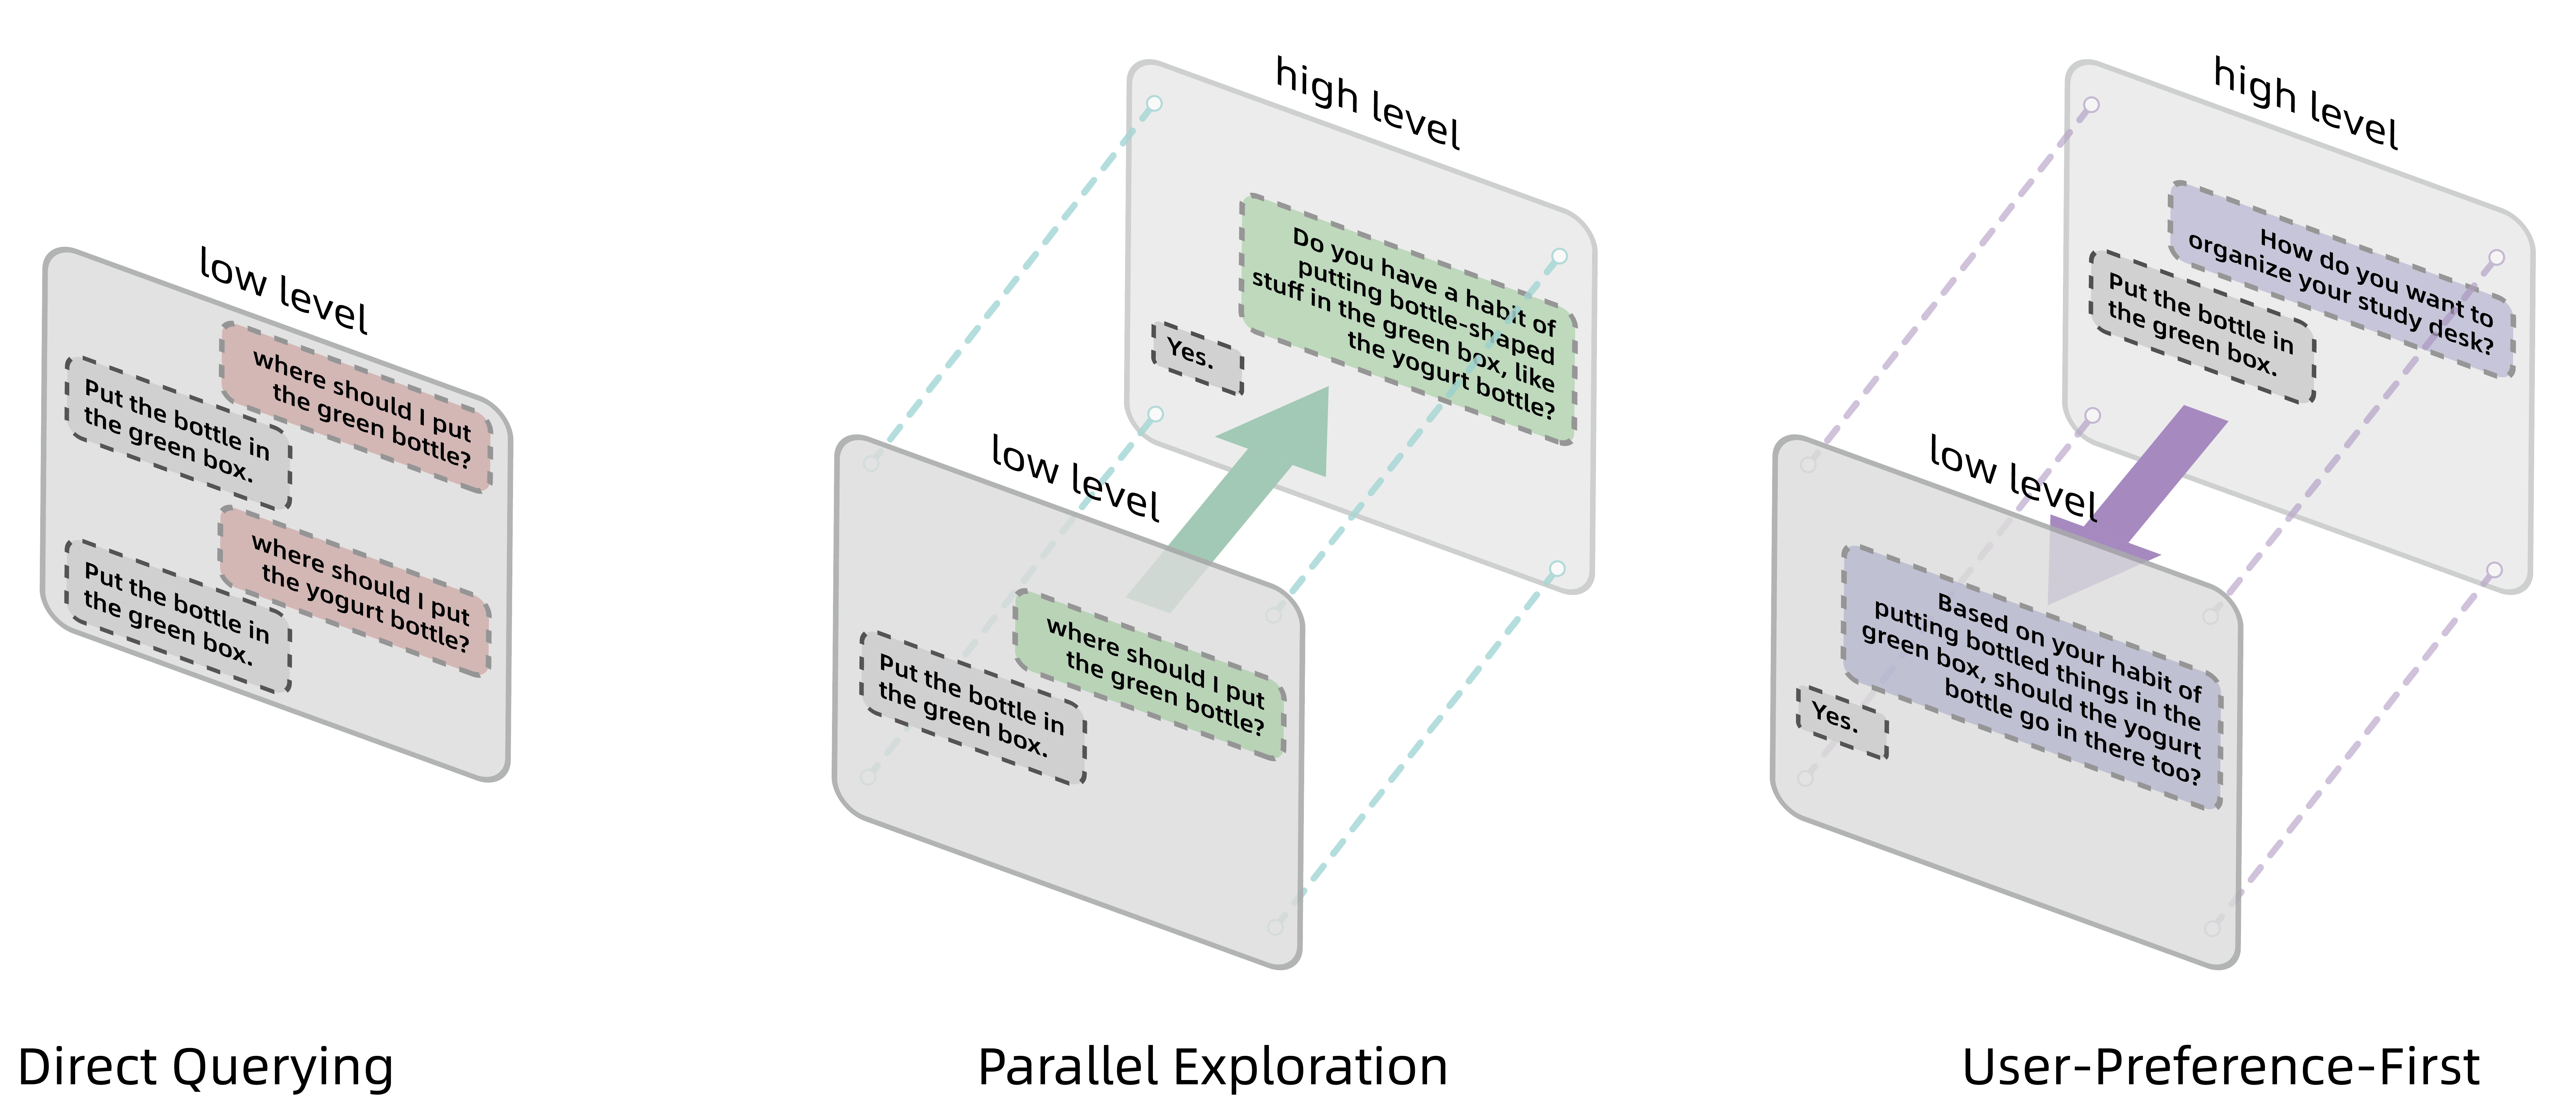
\includegraphics[width=\linewidth]{img/3.3.3.png}
  \caption{Hierarchical coding framework for analyzing questioning strategies. 
  The process begins with knowledge-level annotation, proceeds to intent-level coding, and culminates in the identification of higher-level conversational patterns and strategies.}
  \label{fig:annotation-framework}
\end{figure}


\begin{table}[t]
\centering
\caption{Three questioning patterns with descriptions and representative examples. 
AO = Action-oriented; PE = Preference-eliciting; PS = Preference-summarizing. Arrows ($\rightarrow$) indicate sequence progression.}
\label{tab:patterns}
\begin{tabularx}{\linewidth}{@{} l >{\raggedright\arraybackslash}X >{\raggedright\arraybackslash}X @{}}
\toprule
\textbf{Pattern} & \textbf{Description} & \textbf{Examples} \\
\midrule
\textbf{Direct Querying} & 
All questions are directed toward concrete task operations without proactively considering the user’s preferences; reflects a reactive, surface-level style. &
``The milk won't fit---should I put it on the lower shelf?'' (AO) $\rightarrow$
``Where should I place the small yogurt cups?'' (AO) $\rightarrow$
``Where do the fresh vegetables go?'' (AO) $\rightarrow$
``What should I do if the left side is full?'' (AO) \\
\midrule
\textbf{Parallel Exploration} &
Preference-related questions are interleaved with task-related ones, integrating user needs with procedural decisions. &
``Where should I place this bottle of juice?'' (AO) $\rightarrow$
``So you prefer to keep beverages together on the door, right?'' (PS) $\rightarrow$
``Should I put the apples in the middle drawer?'' (AO) $\rightarrow$
``So overall, you like vegetables stored separately from fruits, correct?'' (PS) \\
\midrule
\textbf{User-Preference-First} &
The sequence begins by eliciting user preferences, which then guide subsequent task decisions. &
``Do you have a preferred way of grouping items in the fridge?'' (PE) $\rightarrow$
``Should drinks go on the door shelf or inside?'' (PE) $\rightarrow$
``Where would you usually place dairy products?'' (AO) $\rightarrow$
``Is this how you normally organize vegetables?'' (AO) \\
\bottomrule
\end{tabularx}
\end{table}


\subsection{Pattern Distribution}
Although some dialogues exhibited within-sequence shifts between questioning patterns, for comparability we adopted a \textit{dominant-pattern} labeling: each dialogue was assigned to the single pattern that best captured its overall trajectory. This choice prioritizes analytical clarity at the dialogue level and enables robust between-task comparisons.

Based on this labeling, we compared distributions across tasks. In the 14 \textit{refrigerator organization} dialogues, 9 sequences (64.3\%) followed \textit{User-Preference-First}, 3 (21.4\%) exhibited \textit{Parallel Exploration}, and 2 (14.3\%) were \textit{Direct Querying}. In contrast, among the 14 \textit{cocktail mixing} dialogues, 2 sequences (14.3\%) adopted \textit{User-Preference-First}, 10 (71.4\%) followed \textit{Parallel Exploration}, and 2 (14.3\%) were \textit{Direct Querying}. These results show that all three patterns appeared in our corpus and were clearly distinguishable at the dialogue level.


\section{System Design and Implementation}
\subsection{From HHI to Robotic Questioning}
In our formative human–human interaction study, we identified three representative questioning patterns. These patterns differ not only in how questions are organized but also in the rhythm of task progression and the extent to which user-provided information is utilized. While these insights can inspire the design of robotic questioning, prior research has not systematically compared these patterns or empirically examined their impact on user perceptions~\cite{cakmak2012designing,hu2024designing,shin2023uncertainty}. To address this gap, we propose a configurable questioning framework that enables robots to flexibly switch between different patterns, thereby allowing us to compare their effects within a unified task environment.

Human conversations often involve a dynamic combination of multiple patterns. For example, users may begin with a \textit{preference-first} approach to establish rules of action, employ \textit{parallel exploration} mid-task to infer operational constraints, and conclude with \textit{confirmatory questioning} to validate preferences. In contrast, for our robotic experiments we abstracted each pattern into a distinct strategy and implemented them separately. This abstraction ensures experimental control and interpretability of results, avoiding potential confounds introduced by mixed patterns. In other words, we treat these three patterns as ``baseline strategies'' for robotic questioning: a stepwise research path that first validates the feasibility and perceptual differences of individual strategies, before extending to more dynamic or hybrid approaches in future work.

\subsection{Strategy Decomposition and Robotic Challenges}

Transferring natural human questioning patterns into robotic systems is far from straightforward. Humans rely on perception, commonsense reasoning, and subtle interactional cues to perform large amounts of implicit inference during dialogue, whereas robots must realize these processes through explicit mechanisms~\cite{strachan2024testing}. In single-turn interactions, the absence of such implicit reasoning may remain largely unnoticed, as the system can often rely on immediate user feedback to proceed. However, in multi-turn questioning, a lack of contextual understanding, discourse consistency, and reasoning over accumulated information becomes a critical bottleneck. 

For instance, humans naturally maintain coherence in dialogue, avoid contradictory information, and integrate incremental exchanges into reasonable inferences. Robots, by contrast, require explicit functional modules to achieve the same outcomes: ensuring contextual consistency, preventing redundancy or contradictions, and reasoning over accumulated knowledge. In other words, abilities that humans accomplish almost ``subconsciously'' must be decomposed into explicit modules to support multi-turn questioning and task execution in robots (see Table~\ref{tab:module_mapping}).

\begin{table}[t]
\centering
\caption{Differences between HHI and robotic deployment in key components.}
\label{tab:module_mapping}
\begin{tabularx}{\linewidth}{lX X l}
\hline
\textbf{Module} & \textbf{Characteristics in HHI} & \textbf{Requirements for Robots} & \textbf{System Module} \\
\hline
Contextual Understanding & Rapidly grasp the task environment by combining perception and commonsense & Requires explicit scene representation and consistency across multi-turn interactions & Scene Understanding \\
\hline
Proactive Questioning & Naturally raises task- and context-sensitive questions & Requires explicit questioning strategies in multi-turn dialogues & Ask Module \\
\hline
Object Grounding & Resolves references using gestures, gaze, or discourse context & Requires robust binding between dialogue content and physical objects & Object Grounder \\
\hline
Preference Extraction & Infers user habits from sparse hints in language and behavior & Requires structured parsing of preferences for consistent multi-turn use & Preference Parser \\
\hline
Clarification Decisions & Instinctively asks follow-up questions to resolve ambiguity & Requires explicit detection of uncertainty and decision on clarification vs. execution & Ambiguity Evaluator \\
\hline
Task Decomposition & Naturally translates intentions into appropriate actions & Requires mapping linguistic feedback into atomic executable actions & Act Module \\
\hline
\end{tabularx}
\end{table}



\begin{itemize}
    \item \textbf{Contextual Understanding:} Humans quickly combine visual, semantic, and commonsense cues to identify task-relevant objects, whereas robots need multi-modal perception and knowledge reasoning to form a coherent scene representation.  
    \item \textbf{Proactive Questioning:} Humans naturally generate context-sensitive questions to elicit critical task information (e.g., implicit constraints, long-term habits). Robots, in turn, must rely on questioning strategies to actively acquire such information and integrate fragmented answers.  
    \item \textbf{Object Grounding:} Ambiguous references (e.g., ``that cup'') are easily resolved by humans using gestures, gaze, or discourse context, while robots require robust object grounding mechanisms to bind language to specific entities.  
    \item \textbf{Preference Extraction:} Humans infer long-term habits from sparse hints (e.g., ``frequently used items are kept nearby''), and adapt to them seamlessly. Robots must instead parse such cues into structured constraints or rules to ensure consistent application across multiple rounds of questioning and execution.  
    \item \textbf{Clarification Decisions:} When facing ambiguous answers, humans instinctively pursue clarification. Robots, however, require explicit ambiguity detection modules to determine whether to continue clarification at the current stage or proceed with execution.  
    \item \textbf{Task Decomposition:} Humans readily translate intentions into actionable steps, whereas robots must map language feedback into atomic actions to guarantee reliable execution after multi-step reasoning.  
\end{itemize}

Beyond these aspects, humans in HHI further leverage multi-modal signals such as facial expressions and prosody to flexibly switch between questioning patterns and to maintain accumulated context through memory. While not the main focus of this work, these phenomena highlight the inherent complexity of natural dialogue.


\subsection{Configurable Questioning Strategies for Learning by Asking Robots}
Inspired by recent advances in robotics and large-scale models \cite{5ramrakhya2025grounding,lawley2024val,huang2023instruct2act}, we propose QUEST (Questioning-based Strategy for Teaching)—a framework designed to endow robots with parameterizable question-asking strategies. This enables systematic comparison and analysis of different inquiry strategies within a unified task environment.

To endow robots with human-like questioning abilities during task execution, it is crucial to ensure that the use of Vision-Language Models (VLMs) remains controllable. Based on observations from human--human interaction (HHI), we first decompose implicit conversational skills into a set of core stages (e.g., scene understanding, information extraction, ambiguity handling), and abstract these into explicit functional requirements for robotic systems. Unlike humans, who accomplish these processes subconsciously, robots require explicit mechanisms to support each stage. However, adopting end-to-end free generation directly would easily lead to uncontrollable outputs.

To address this challenge, we propose the modular framework \textbf{QUEST}. On the one hand, modularization ensures that the output of each step is constrained by structured intermediate representations and decision checkpoints, thereby guaranteeing consistency and controllability across modules. On the other hand, modules can be flexibly combined and configured to support different questioning patterns and task demands. In implementation, we construct the VLM as a \textit{toolbox}, where controlled invocations are used to meet functional requirements. Table~\ref{tab:module_mapping} summarizes the mapping from natural behaviors in HHI, through robotic deployment requirements, to their modular implementation in QUEST.

Figure~\ref{fig:system-architecture} illustrates the overall architecture of QUEST, which consists of three main components: \textit{Ask}, \textit{Think}, and \textit{Act}. The framework simulates the process of progressively clarifying and accumulating task-relevant knowledge through questioning until successful task completion. Its operation is driven by the \textit{Ask--Think--Act} loop: during the \textit{Ask} phase, the robot generates questions based on the environment and configured strategy to acquire missing task-critical information; in the \textit{Think} phase, the system parses and reasons over user answers, including information extraction, entity grounding, and ambiguity detection, and, if necessary, returns to the \textit{Ask} phase for follow-up questions; once the information becomes sufficient and unambiguous, the loop transitions to the \textit{Act} phase, where high-level intentions are converted into atomic actions that drive robot execution.

\begin{figure*}[t]
  \centering
  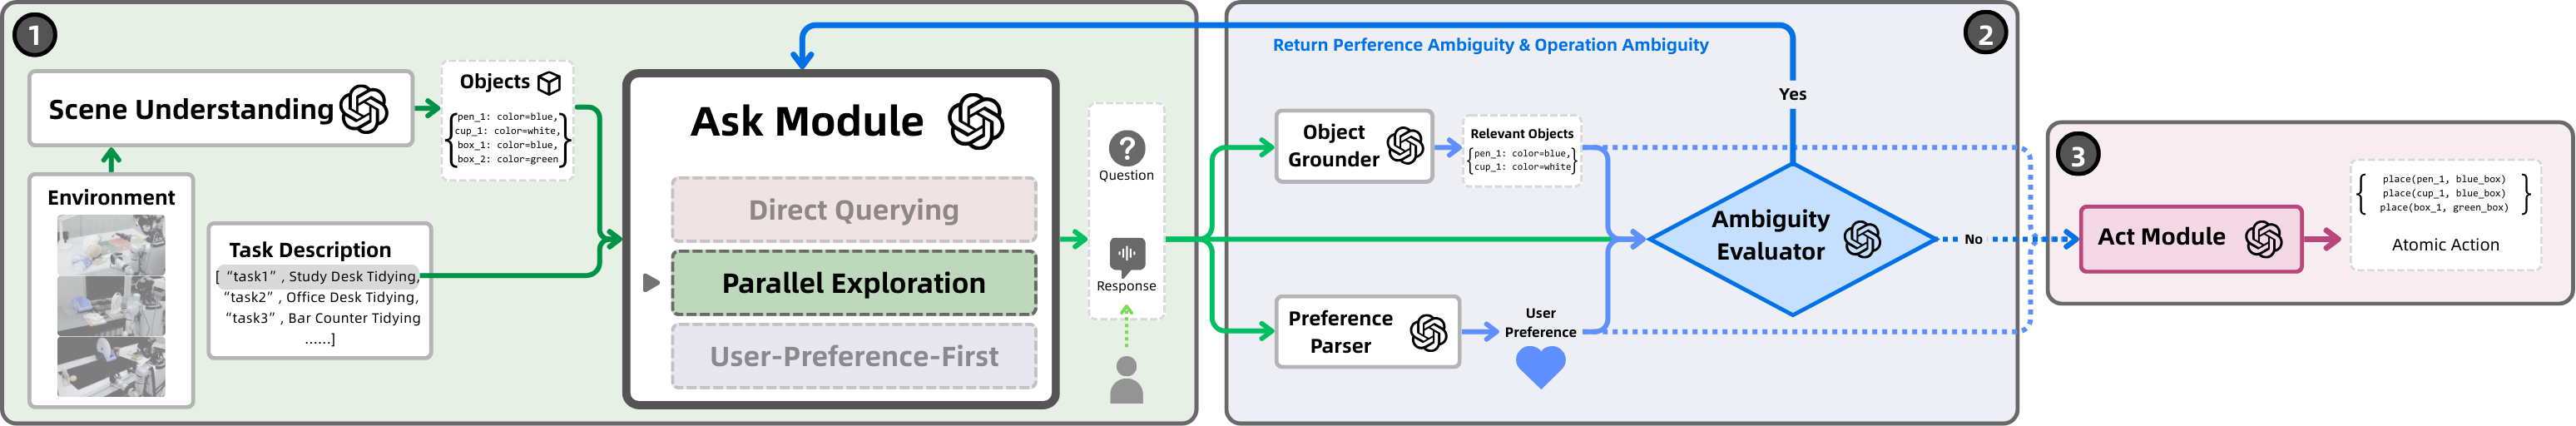
\includegraphics[width=\textwidth]{img/system.png}
  \caption{Overview of our system architecture. (1) The \textit{Scene Understanding} module interprets the environment and task description to extract objects. (2) The \textit{Ask Module} deploys questioning strategies (Direct Querying, Parallel Exploration, User-Preference-First) and interfaces with ambiguity evaluation through object grounding and preference parsing. (3) The \textit{Act Module} executes atomic actions once ambiguities are resolved.}
  \label{fig:system-architecture}
\end{figure*}

In the following sections, we introduce the design and function of six key modules in QUEST. For each module, we provide illustrative input–output examples to demonstrate its role within the framework. All modules are implemented as independent GPT-based subprograms, formally defined as follows.


\subsubsection{Scene Understanding}

The Scene Understanding module constructs a structured representation of the environment from multimodal perception and task context. It integrates visual inputs (e.g., RGB-D frames) with the task description to identify objects, their attributes, and spatial relations. The module outputs a set of candidate entities that can be referenced in later dialogue. For example, in a desk tidying scenario, Scene Understanding may detect \{pen\_1, pen\_2, notebook\_1, cup\_1\} along with their attributes (e.g., color, type).

\begin{figure}[H]
  \centering
  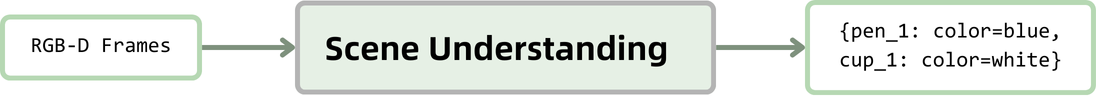
\includegraphics[width=0.75\linewidth]{img/4.3.1.png}
  %\caption{Scene Understanding }
  %\label{scene understanding}
\end{figure}

\subsubsection{Ask Module}
The \textit{Ask Module} generates the robot’s questions by combining the structured scene representation, the task description, and ambiguity signals from the interaction. Unlike unconstrained language generation, it is explicitly parameterized by a single questioning strategy (User-Preference-First, Parallel Exploration, or Direct Querying; see Figure~\ref{fig:system-architecture}), ensuring consistency throughout the dialogue.  When \textit{preference ambiguity} is detected, the module produces high-level questions to elicit organizational rules (e.g., \textit{``Do you usually group stationery together?''}). When \textit{operational ambiguity} arises, it formulates concrete placement questions (e.g., \textit{``Should I put this notebook into the left drawer?''}). By enforcing concise, single-sentence outputs and restricting references to simple object names, the \textit{Ask Module} provides a unified yet configurable interface for instantiating distinct questioning strategies, thereby enabling controlled comparison within the QUEST framework.

\begin{figure}[H]
  \centering
  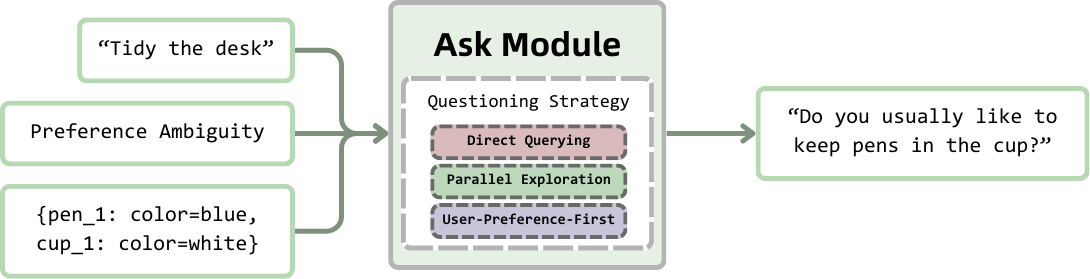
\includegraphics[width=0.75\linewidth]{img/4.3.2.png}
  %\caption{Ask Module}
\end{figure}


\subsubsection{Object Grounder}

The \textit{Object Grounder} links user utterances to concrete objects detected in the scene. It takes candidate entities from Scene Understanding together with linguistic references from the Ask--Think loop, and resolves them into unique object IDs. The module must handle vague or underspecified expressions such as \textit{``this cup''} or \textit{``these notebooks''}, using spatial context and attributes to disambiguate. For instance, the phrase \textit{``these two notebooks''} may be grounded to \texttt{notebook\_1} and \texttt{notebook\_2}, while \textit{``the cup on the left''} is bound to \texttt{cup\_3}.

\begin{figure}[H]
  \centering
  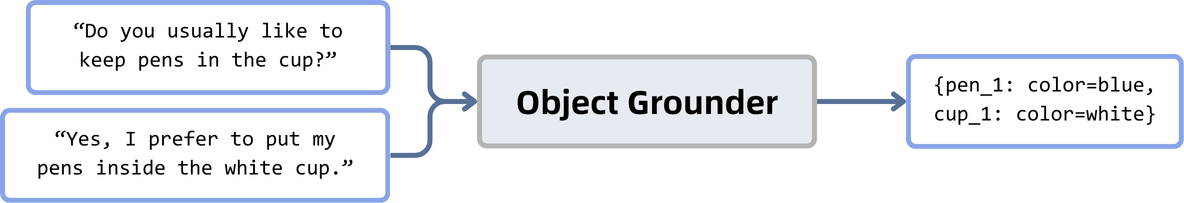
\includegraphics[width=0.75\linewidth]{img/4.3.3.png}
  %\caption{Object Grounder}
\end{figure}


\subsubsection{Preference Parser}

The \textit{Preference Parser} converts user responses into structured preferences that can be reused across the interaction. Unlike humans, who can effortlessly infer rules and constraints from implicit cues, robots require an explicit mechanism to formalize them. In QUEST, preferences are represented in three dimensions:  

\begin{itemize}
  \item \textbf{Operational preferences} — These capture direct instructions about how to handle individual objects or categories. They are typically tied to immediate actions and provide the system with concrete placement or grouping decisions.
  \item \textbf{General principles} — These represent higher-level organizational rules that generalize across multiple contexts. They guide the robot toward consistent long-term behavior, rather than just solving a single instance of ambiguity.
  \item \textbf{Forbiddens} — These encode explicit prohibitions that constrain the robot’s choices. By preventing certain actions or placements, they ensure that the system respects the user’s boundaries and avoids undesired outcomes.
\end{itemize}

\begin{figure}[H]
  \centering
  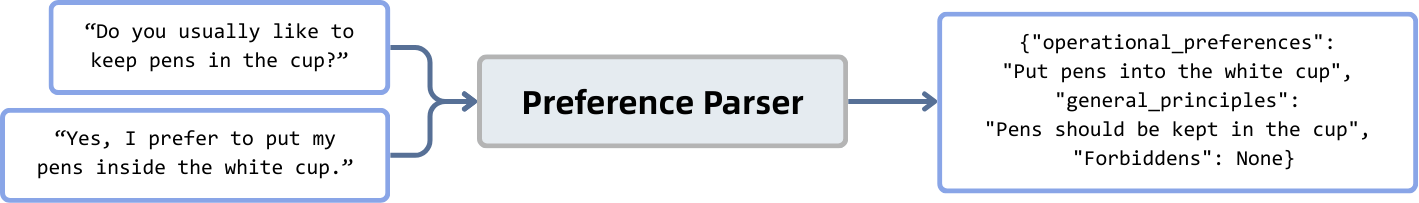
\includegraphics[width=0.75\linewidth]{img/4.3.4.png}
  %\caption{Preference Parser}
\end{figure}


\subsubsection{Ambiguity Evaluator}
The \textit{Ambiguity Evaluator} assesses whether the information currently available is sufficient for the robot to proceed with execution, or whether additional clarification is required. It integrates three streams of input: the relevant objects detected in the scene, the dialogue history between the robot and the user, and the structured preferences produced by the \textit{Preference Parser}. Based on these sources, the module determines whether a target can be uniquely operated on, or if further questioning is needed to resolve uncertainty.  

Rather than relying on implicit inference as humans do, the robot requires an explicit mechanism to guard against premature or erroneous actions. The \textit{Ambiguity Evaluator} therefore functions as a decision checkpoint in the interaction loop. Its output follows a structured format, specifying whether the object is operable, the type of ambiguity if one is present, and the missing or conflicting information that prevents execution. In this way, the module ensures that the system either continues smoothly to the \textit{Act Module} or returns to the \textit{Ask Module} for clarification.

\begin{figure}[H]
  \centering
  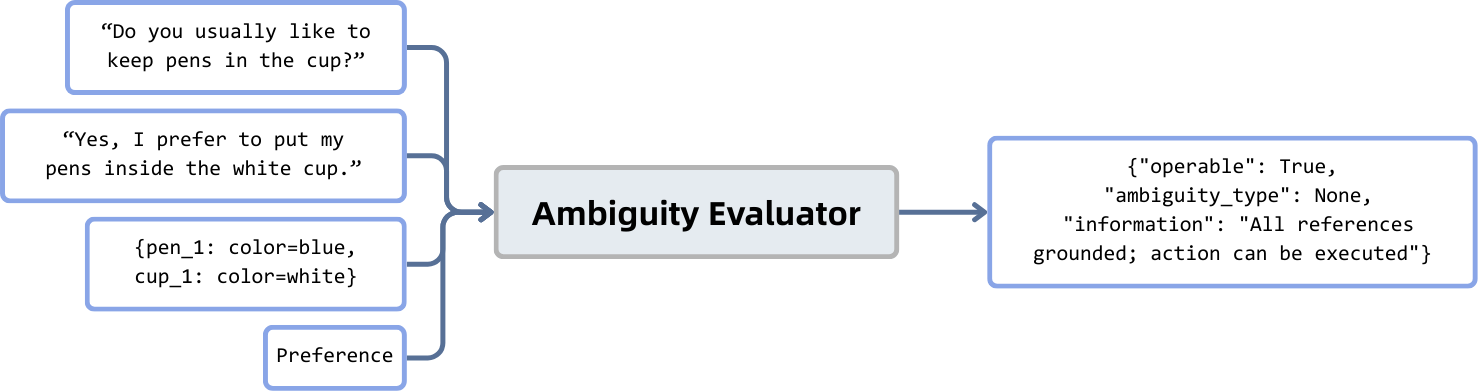
\includegraphics[width=0.75\linewidth]{img/4.3.5.png}
  %\caption{Ambiguity Evaluator}
\end{figure}

\subsubsection{Act Module}
The \textit{Act Module} is responsible for converting high-level dialogue outcomes into executable actions on the robot. Drawing on contextual inputs—including the set of relevant objects identified in the scene and the structured preferences parsed from user responses—the module generates atomic operations that can be directly executed. These actions follow a predicate--argument form, such as \texttt{place(object, location)}, \texttt{group(object\_a, object\_b)}, or \texttt{remove(object)}, which serve as the interface between language understanding and low-level control.  
The \textit{Act Module} is responsible for converting high-level dialogue outcomes into executable actions on the robot. Drawing on contextual inputs—including the set of relevant objects identified in the scene and the structured preferences parsed from user responses—the module generates atomic operations that can be directly executed. These actions follow a predicate--argument form, such as \texttt{place(object, location)}, \texttt{group(object\_a, object\_b)}, or \texttt{remove(object)}, which serve as the interface between language understanding and low-level control.  

\begin{figure}[H]
  \centering
  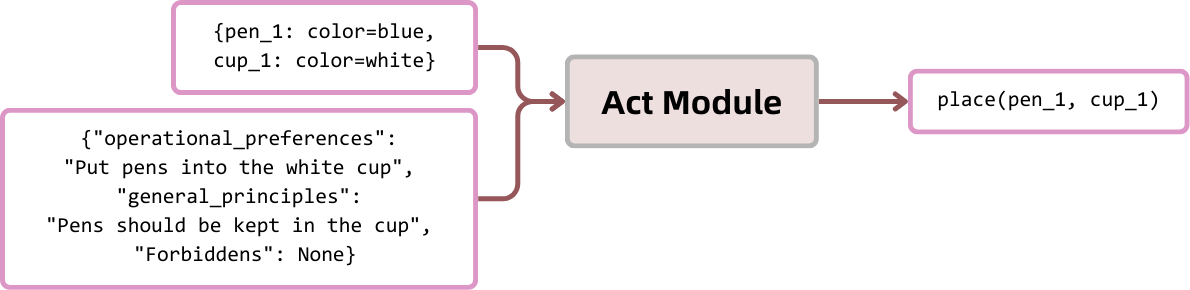
\includegraphics[width=0.75\linewidth]{img/4.3.6.png}
  %\caption{Act Module}
\end{figure}


\subsection{Deployment of Questioning Strategies}
In QUEST, the three questioning strategies are implemented through parameterized prompts in the Ask Module. Inspired by the patterns observed in our HHI study, we designed concise templates that constrain the scope of questions, the way follow-ups are posed, and the granularity of operations. This design allows the same VLM to be flexibly instantiated under different strategies, while ensuring that each strategy remains consistent across an entire interaction. Below we summarize the core prompt logic of each strategy.

\paragraph{Direct Querying.}  
This strategy focuses exclusively on immediate, localized operations. The prompt constrains the system to generate short, specific questions tied to a single object or position, without attempting to probe or summarize user preferences. This yields a reactive and fine-grained interaction style that maximizes clarity but does not generalize beyond the immediate step. Typical questions include \textit{``Should I place this blue pen in the left drawer?''} or \textit{``Does this book belong on the top shelf?''}  

\noindent\textbf{Prompt:} ``You are a home service robot using the `Direct Querying' questioning strategy. Focus exclusively on immediate, localized operations. Always ask short, specific questions about a single object or position, without attempting to probe or summarize user preferences. Rule for question generation: (1) Select one unoperated item; (2) Ask a concise, direct question about its immediate placement or handling; (3) Ensure no repetition; (4) Output one concise question.''

\paragraph{Parallel Exploration.}  
This strategy begins by eliciting high-level organizational rules or user habits before turning to individual objects. Instead of following a fixed alternation pattern, the prompt encourages the system to flexibly switch between object-specific questions and higher-level rules, depending on the current state of the dialogue. When task progress is needed, the system generates a concrete action-oriented question about a single object; when sufficient evidence has accumulated, it attempts to generalize and confirm a broader rule. For instance, the robot might ask \textit{``Should I put this notebook into the drawer?''} and later follow up with \textit{``Based on what we have done so far, do you prefer to keep all stationery together?''}  

\noindent\textbf{Prompt:} ``You are a home service robot using the `Parallel Exploration' questioning strategy. Alternate flexibly between concrete questions about specific items and higher-level questions about possible rules. Always keep questions short and natural. Rule for question generation: (1) When task progress is needed, ask a direct question about a specific item; (2) When enough evidence has accumulated from prior actions, propose a general rule and ask the user to confirm it; (3) Ensure no repetition; (4) Output one concise question.''


\paragraph{User-Preference-First.}  
This strategy prioritizes the elicitation of high-level organizational rules or user habits before addressing specific objects. The prompt guides the system to begin with abstract questions about preferences, which then serve as a foundation for subsequent operational decisions. Compared to other strategies, it emphasizes early establishment of global rules, thereby reducing the need for repeated clarifications later in the task. For example, the system may ask \textit{``Do you usually distinguish between frequently used and rarely used items?''} or \textit{``When tidying the desk, do you prefer to separate study materials from daily supplies?''}  

\noindent\textbf{Prompt:} ``You are a home service robot using the `User-Preference-First' questioning strategy. Begin by eliciting high-level organizational rules or user habits before asking about specific objects. These abstract preferences should then serve as the foundation for subsequent operational questions. Rule for question generation: (1) If no general principle has been established, ask a broad question to uncover a high-level preference; (2) Once a principle is available, apply it to specific items or categories with direct questions; (3) Ensure no repetition; (4) Output one concise question.''


\subsection{Robot Platform}
We employed a Unitree G1-EDU humanoid robot, which provides 23–43 Degrees of Freedom (DOF), including articulated legs, a waist joint, and dual 5-DOF arms that can be optionally extended with dexterous multi-fingered hands. The platform integrates a depth camera, 3D LiDAR, and a four-microphone array for multimodal perception, with onboard computation supported by an NVIDIA Jetson Orin module. Speech input is captured via the microphone array and transcribed using automatic speech recognition. These multimodal inputs are processed by a vision–language model (OpenAI’s \texttt{gpt-5-mini-2025-08-07}) with tool usage through Python. To ensure a smooth user experience centered on questioning strategies, we selected the model configuration to balance response latency with reasoning capability.


\section{User Study}
We conduct an in-person user study (N=18) to examine how varying a robot’s questioning strategy through the QUEST system prompts shapes users’ perceptions and interaction experience in household tasks. 

\subsection{Study Design}
We employed a within-subjects design, in which all participants experienced all three task scenarios (\textit{desk tidying}, \textit{office desk tidying}, \textit{bar counter tidying}) and all three questioning strategies (\textit{Direct Querying}, \textit{Parallel Exploration}, \textit{User-Preference-First}). Each participant thus completed nine trials in total, with the order of scenarios and strategies counterbalanced using a Latin square. All scenarios were designed with comparable complexity (approximately 10--12 items and 2--3 storage spaces) to minimize potential confounds. The robot was operated via a Wizard-of-Oz setup to ensure consistent execution across conditions, thereby isolating the effects of the questioning strategies. Figure~\ref{fig:strategies} provides an overview of the three questioning strategies across the three task scenarios.


\begin{figure}[t]
    \centering
    \includegraphics[width=\linewidth]{img/user-study.png}
    \caption{Illustration of the three questioning strategies (\textit{Direct Querying}, \textit{Parallel Exploration}, \textit{User-Preference-First}) across three task scenarios (\textit{study desk tidying}, \textit{office desk tidying}, \textit{bar counter tidying}).}
    \label{fig:strategies}
\end{figure}

\subsection{Tasks}
We design three representative household tidying tasks, each set up as a long-term task with multiple sub-goals and inherent ambiguity. The study is conducted in a lab environment resembling a household setting: the required items (full lists are provided in Appendix~\ref{app:items}) are placed on a central table, and a dual-arm humanoid robot is positioned next to it. Participants’ goal is not to complete the tasks themselves but to \textit{teach the robot} how to perform them. A task is considered complete once the robot can continue without further questioning.  

\textbf{Study Desk Tidying.} Participants teach the robot to organize a cluttered study desk. The goal is to achieve a neat and usable workspace, while individual preferences differ in how items are categorized or whether frequently used objects remain accessible.  

\textbf{Office Desk Tidying.} Participants teach the robot to tidy a desk piled with various objects. The goal is to obtain a clean working surface, while user preferences vary in book arrangement and the use of storage utilities.  

\textbf{Bar Counter Tidying.} Participants teach the robot to organize a cluttered bar counter. The goal is to achieve a clean and safe layout, while user preferences differ in how tableware is arranged and whether tools remain within reach.  
 
\subsection{Apparatus}
We use a dual-arm humanoid robot system in the study. The robot is controlled by a PC running Linux, and an additional laptop is provided for participants to complete questionnaires. The robot is positioned on one side of the table, with participants seated in a designated chair on the opposite side. The field of view of the robot’s camera is marked on the floor, and participants are instructed to remain outside this area before the study begins.  

The experimenter sits at the control PC with direct access to the robot’s emergency stop button and can start or stop the study tasks at any time. To ensure reliable execution of low-level actions, the robot is teleoperated in real time through a VR interface: the experimenter wears a VR headset and controllers, mapping natural arm and hand movements to the robot to achieve precise and flexible manipulation.  Participants interact with the robot using natural language. A microphone array captures speech, which is transcribed and passed to the questioning and teleoperation system to generate context-aware responses.


 

\subsection{Procedure}
After a general introduction to the study and the robot, participants were informed about the study purpose, potential risks, and their rights, and provided written informed consent. The experimenter also familiarized participants with the experimental environment and objects, and reminded them of essential safety instructions (e.g., keeping a safe distance from the robot and avoiding unexpected contact during its movements). Participants then completed a demographic questionnaire, the Affinity for Technology Interaction scale (ATI), and the Negative Attitudes toward Robots Scale (NARS). 

Before the main study, we conducted a standardized \textit{practice trial} in which participants guided the robot through its active questioning to place a bottle into a box. This familiarized participants with the “robot-asks–user-responds” interaction pattern, including answering clarification questions, explaining preferences, and correcting robot actions. Once participants indicated they were comfortable with the interaction, the main study began.  

In the main study, each participant completed three tidying tasks. For each trial, the experimenter prepared the initial environment, and participants stood near the desk or bar counter while teaching the robot to complete the task by answering its questions. No strict time limit was imposed. After each trial, participants filled out a short questionnaire on a separate computer, after which the environment was reset and switched to another questioning strategy. After completing all three tasks, participants took part in a semi-structured interview focusing on their perceived differences between strategies, their preferences and trade-offs, and whether the robot had accurately captured their preferences.


\subsection{Measures and Analysis}
We administered three questionnaires after each task round. First, we used the original NASA-TLX scale~\cite{hart1988development} to evaluate participants’ perceived workload, covering six dimensions: mental demand, physical demand, temporal demand, effort, performance, and frustration. Second, we adopted the Perceived System Curiosity Scale (PSC)~\cite{conf/chi/LeusmannVB0M25}, which includes three subscales—Explorative Curiosity (PSC-E), Investigative Curiosity (PSC-I), and Social Curiosity (PSC-S)—to capture how participants perceived the robot’s “curious” behavior. We chose PSC because prior HRI studies demonstrated that robots displaying curiosity are often perceived as more engaging, human-like, and enjoyable interaction partners, and users tend to prefer teaching or collaborating with such robots over non-curious ones~\cite{8leusmann2025investigating}. Finally, we used the General Self-Efficacy Scale (GSE)~\cite{schwarzer1995generalized} to assess participants’ confidence and sense of control during the teaching process. By repeating these measures after each round, we were able to track how the three questioning strategies influenced subjective experience across different scenarios.



Besides, we logged the complete interaction history between participants and the robot. Robot-side events were categorized into four activity states—\textit{Ask-Confirm}, \textit{Act}, \textit{Fail}, and \textit{Wait}—from which we derived quantitative metrics. Specifically, we modeled event sequences as row-normalized state-transition matrices to examine policy-dependent procedural dynamics (see Section~6.1.1).

For qualitative feedback, after completing all three task rounds, each participant took part in a semi-structured interview lasting about fifteen minutes. The interview questions focused on their preferences and trade-offs between the questioning strategies, their subjective evaluation of the quality and timing of questions. All interviews were audio-recorded, transcribed, and analyzed thematically using Atlas.ti 5. Two researchers independently coded approximately 20\% of the material, after which the codes were discussed with two additional researchers to develop a unified codebook and thematic framework. The remaining material was coded by one researcher, and the final results were validated through team discussions.


\subsection{Participants}
We recruited 18 participants (15 female, 3 male). To reduce novelty effects and focus the study on perceptions of the interaction rather than the robot itself, we aimed to recruit participants with relatively high technological affinity and, where possible, prior HRI experience. Participants’ mean age was 23.8 years ($SD = 6.1$, $min = 21$, $max = 45$). In terms of education, 2 held a doctoral degree, 11 a master’s degree, and 5 a bachelor’s degree. To capture baseline individual differences, we used the Affinity for Technology Interaction scale (ATI)~\cite{franke2019personal}, with an average score of $M = 3.16$ ($SD = 0.7$). We also administered the Negative Attitudes toward Robots Scale (NARS)~\cite{syrdal2009negative}, measuring participants’ negative attitudes toward (S1) interaction with robots ($M = 1.99$, $SD = 0.53$), (S2) social influence of robots ($M = 3.16$, $SD = 0.7$), and (S3) emotions in interaction with robots ($M = 2.59$, $SD = 0.75$).  Regarding prior experience with robots, 6 participants had interacted with robots more than seven times, 10 had interacted 1–7 times, and 2 had never interacted with a robot. Reported types of robots included robotic arms (5), humanoid robots (8), social robots (6), and household robots such as vacuum cleaners or voice assistants (16).  We additionally recorded participants’ task familiarity on a 7-point scale: they reported a mean frequency of 4.0 ($SD = 1.64$) for tidying desks or organizing items over the past six months, and a mean self-rated proficiency of 4.11 ($SD = 1.57$). This baseline data allowed us to control for differences in everyday experience across the three task scenarios.  


\section{Results}

\subsection{Quantitative Interaction Data Analysis}
We verified that the three prompting policies, when deployed on the VLM-controlled robot, produced distinct interaction dynamics. Two core authors annotated all robot-only event states, yielding 413 sequences for \textit{Direct-Querying}, 253 for \textit{User-Preference-First}, and 373 for \textit{Parallel-Exploration}. Robot-only event sequences were modeled across four states—\textit{Ask-Confirm}, \textit{Act}, \textit{Preference-Elicit}, and \textit{Preference-Confirm} (where \textit{Act} denotes a physical operation by the robot)—as row-normalized 4$\times$4 transition matrices for each Participant $\times$ Policy (Fig.~\ref{fig:transition-matrices}). Following Leusmann et al.’s event-transition procedure~\cite{conf/chi/LeusmannVB0M25}, we conducted a repeated-measures multivariate test (Pillai’s trace) with Policy as the within-subject factor and participant IDs as a random effect, using all matrix elements as dependent variables.  

The multivariate effect of Policy was significant (Pillai’s trace = 0.336, $F$(3,32) = 5.392, $p <$ .001). Holm-corrected post-hoc tests further isolated six diagnostic transitions that differed reliably across policies: \textit{Act$\rightarrow$Ask-Confirm}, \textit{Act$\rightarrow$Preference-Elicit}, \textit{Act$\rightarrow$Preference-Confirm}, \textit{Preference-Elicit$\rightarrow$Act}, \textit{Preference-Elicit$\rightarrow$Preference-Elicit}, and \textit{Preference-Confirm$\rightarrow$Act}. These findings establish systematic, policy-dependent state-transition patterns.  

Inspection of the transition matrices corroborated these statistical results. Compared to \textit{Direct-Querying}, both \textit{User-Preference-First} and \textit{Parallel-Exploration} reduced the \textit{Act$\rightarrow$Ask-Confirm} transition ($-0.56$/$-0.69$) and increased preference-related flows such as \textit{Preference-Elicit$\rightarrow$Act} ($+0.26$/$+0.29$). \textit{Parallel-Exploration} additionally amplified \textit{Act$\rightarrow$Preference-Elicit} ($+0.29$). In contrast, \textit{Direct-Querying} exhibited a tight \textit{Ask-Confirm$\leftrightarrow$Act} loop (0.95/1.00), whereas the other two policies routed actions through preference states and suppressed immediate returns to confirmation (\textit{Act$\rightarrow$Ask-Confirm}: 0.44 and 0.31).  

For robustness, a pooled homogeneity $\chi^2$ test on Laplace-smoothed matrices also rejected the null hypothesis of equality across policies ($\chi^2$ = 465.35, $df$ = 30, $p <$ .001). All substantive claims, however, are based on the unsmoothed individual matrices.  

\textit{Interpretation.} The deployed policies encode qualitatively distinct procedural strategies: \textit{Direct-Querying} favors an immediate confirm$\rightarrow$act$\rightarrow$confirm loop; \textit{User-Preference-First} channels actions through preference elicitation and confirmation; and \textit{Parallel-Exploration} interleaves acting with preference-related questioning. These patterns demonstrate that the policies achieved clear behavioral separation when executed on the robot, rather than merely reflecting superficial prompt variations.

\begin{figure}[t]
    \centering
    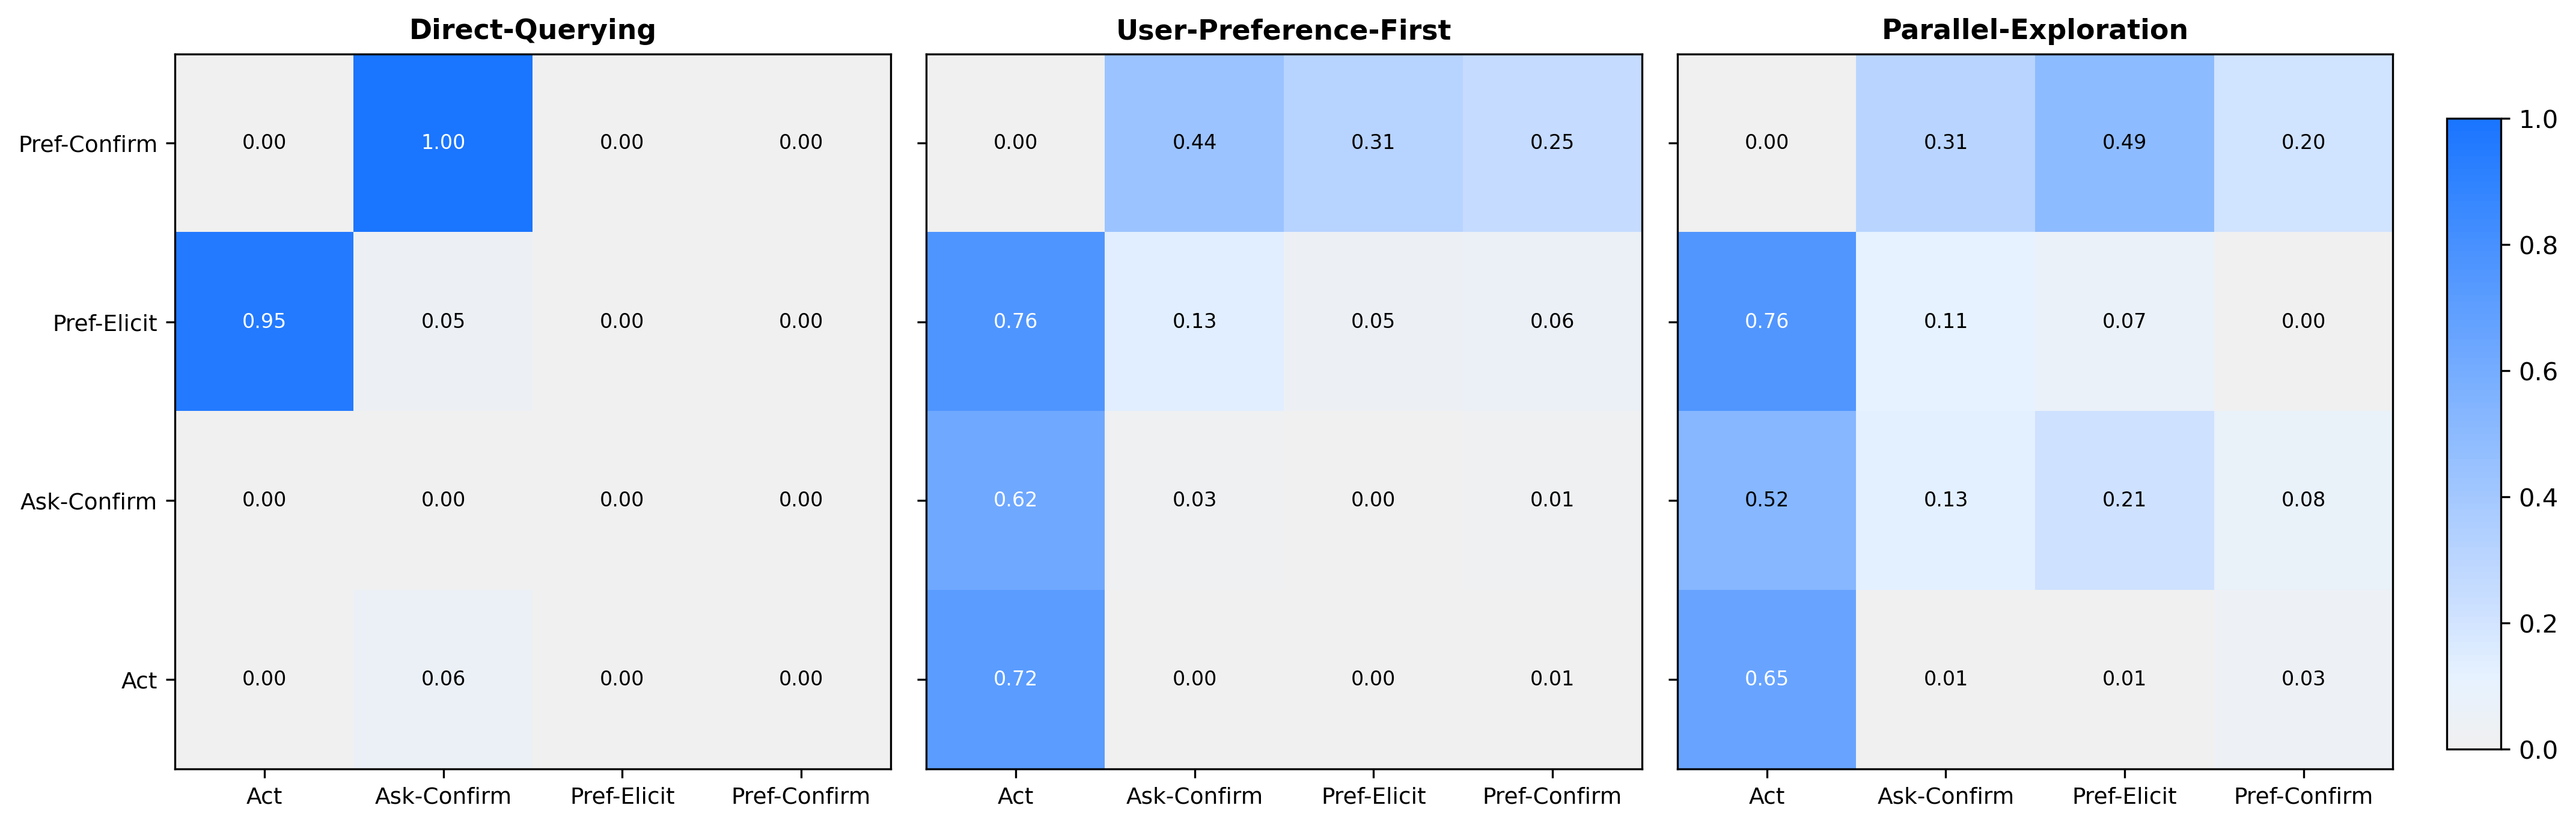
\includegraphics[width=\linewidth]{img/transition-matrices.png}
    \caption{Row-normalized state-transition matrices across the four event states (\textit{Ask-Confirm}, \textit{Act}, \textit{Preference-Elicit}, \textit{Preference-Confirm}) for each questioning policy. \textit{Direct-Querying} shows a tight \textit{Ask-Confirm$\leftrightarrow$Act} loop, whereas \textit{User-Preference-First} and \textit{Parallel-Exploration} route actions through preference states.}
    \label{fig:transition-matrices}
\end{figure}


\subsection{Questionnaire Results}

\begin{table}[ht]
\centering
\caption{Statistical analysis results of all questionnaires (S1 = Direct Querying, S2 = Parallel Exploration, and S3 = User-Preference-First).}
\begin{tabular}{lccccc}
\hline
Measure & W & $p_{norm}$ & $F$ / $\chi^2$ & $p$ & $\eta^2$ / partial $\eta^2$ \\
\hline
\textbf{GSE} & & & & & \\
GSE & 0.920 & .002 & 0.254 & .777 & .009 \\
\hline
\textbf{PSC} & & & & & \\
PSCE        & 0.940 & .009 & 3.401  & .063 & .167 \\
PSCI        & 0.952 & .030 & 6.838  & $<.01$\textsuperscript{*} & .287 \\
PSCS        & 0.961 & .079 & 7.235  & $<.01$\textsuperscript{*} & .299 \\
PSC         & 0.942 & .011 & 7.597  & $<.01$\textsuperscript{*} & .309 \\
\hline
\textbf{NASA-TLX} & & & & & \\
Mental demand   & 0.922 & .002 & 6.644  & $<.05$\textsuperscript{*} & .185 \\
Physical demand & 0.813 & .000 & 0.821  & .663 & .023 \\
Temporal demand & 0.873 & .000 & 1.163  & .559 & .032 \\
Performance     & 0.916 & .001 & 0.982  & .612 & .027 \\
Effort          & 0.940 & .010 & 12.516 & $<.01$\textsuperscript{*} & .348 \\
Frustration     & 0.899 & .000 & 7.609  & $<.05$\textsuperscript{*} & .211 \\
NASA-TLX        & 0.962 & .640 & 4.515  & $<.05$\textsuperscript{*} & .210 \\
\hline
\end{tabular}
\end{table}

\subsubsection{Raw NASA-TLX}
We first tested the normality of the overall NASA-TLX scores. The results indicated that the data under all three strategy conditions followed a normal distribution (Shapiro–Wilk, $p > .05$). Therefore, we conducted a repeated-measures ANOVA. The analysis revealed a significant main effect of strategy on the overall workload ($F(2,34) = 4.52, p < .05$, partial $\eta^2 = .21$), suggesting that different strategies influenced participants’ perceived workload.

We then examined the six subscales separately. Since most of them did not satisfy the normality assumption, we applied non-parametric Friedman tests. The results showed significant effects of strategy on Mental Demand ($\chi^2(2) = 6.64, p < .05$), Effort ($\chi^2(2) = 12.52, p < .01$), and Frustration ($\chi^2(2) = 7.61, p < .05$). In contrast, no significant differences were observed for Physical Demand ($\chi^2(2) = 0.82, p = .663$), Temporal Demand ($\chi^2(2) = 1.16, p = .559$), or Performance ($\chi^2(2) = 0.98, p = .612$).


\begin{figure*}[t]
    \centering
    \begin{subfigure}{0.14\linewidth}
        \centering
        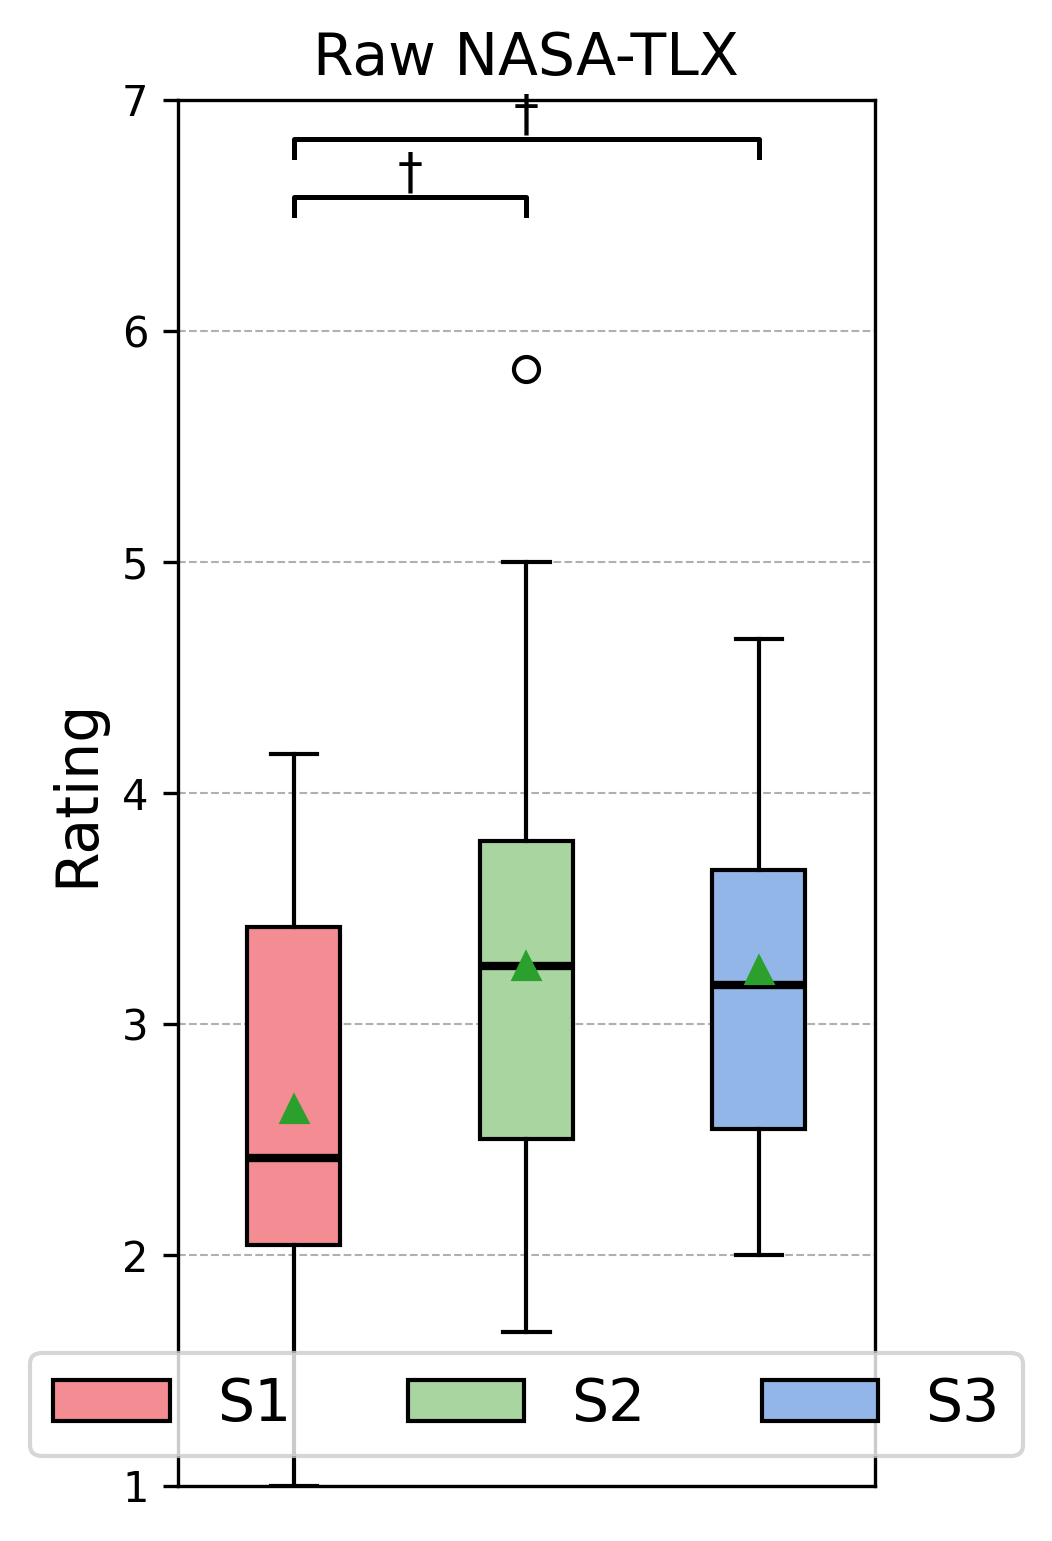
\includegraphics[height=4.7cm]{img/nasa_tlx.png}
        \caption{Raw NASA-TLX}
    \end{subfigure}
    \hfill
    \begin{subfigure}{0.58\linewidth}
        \centering
        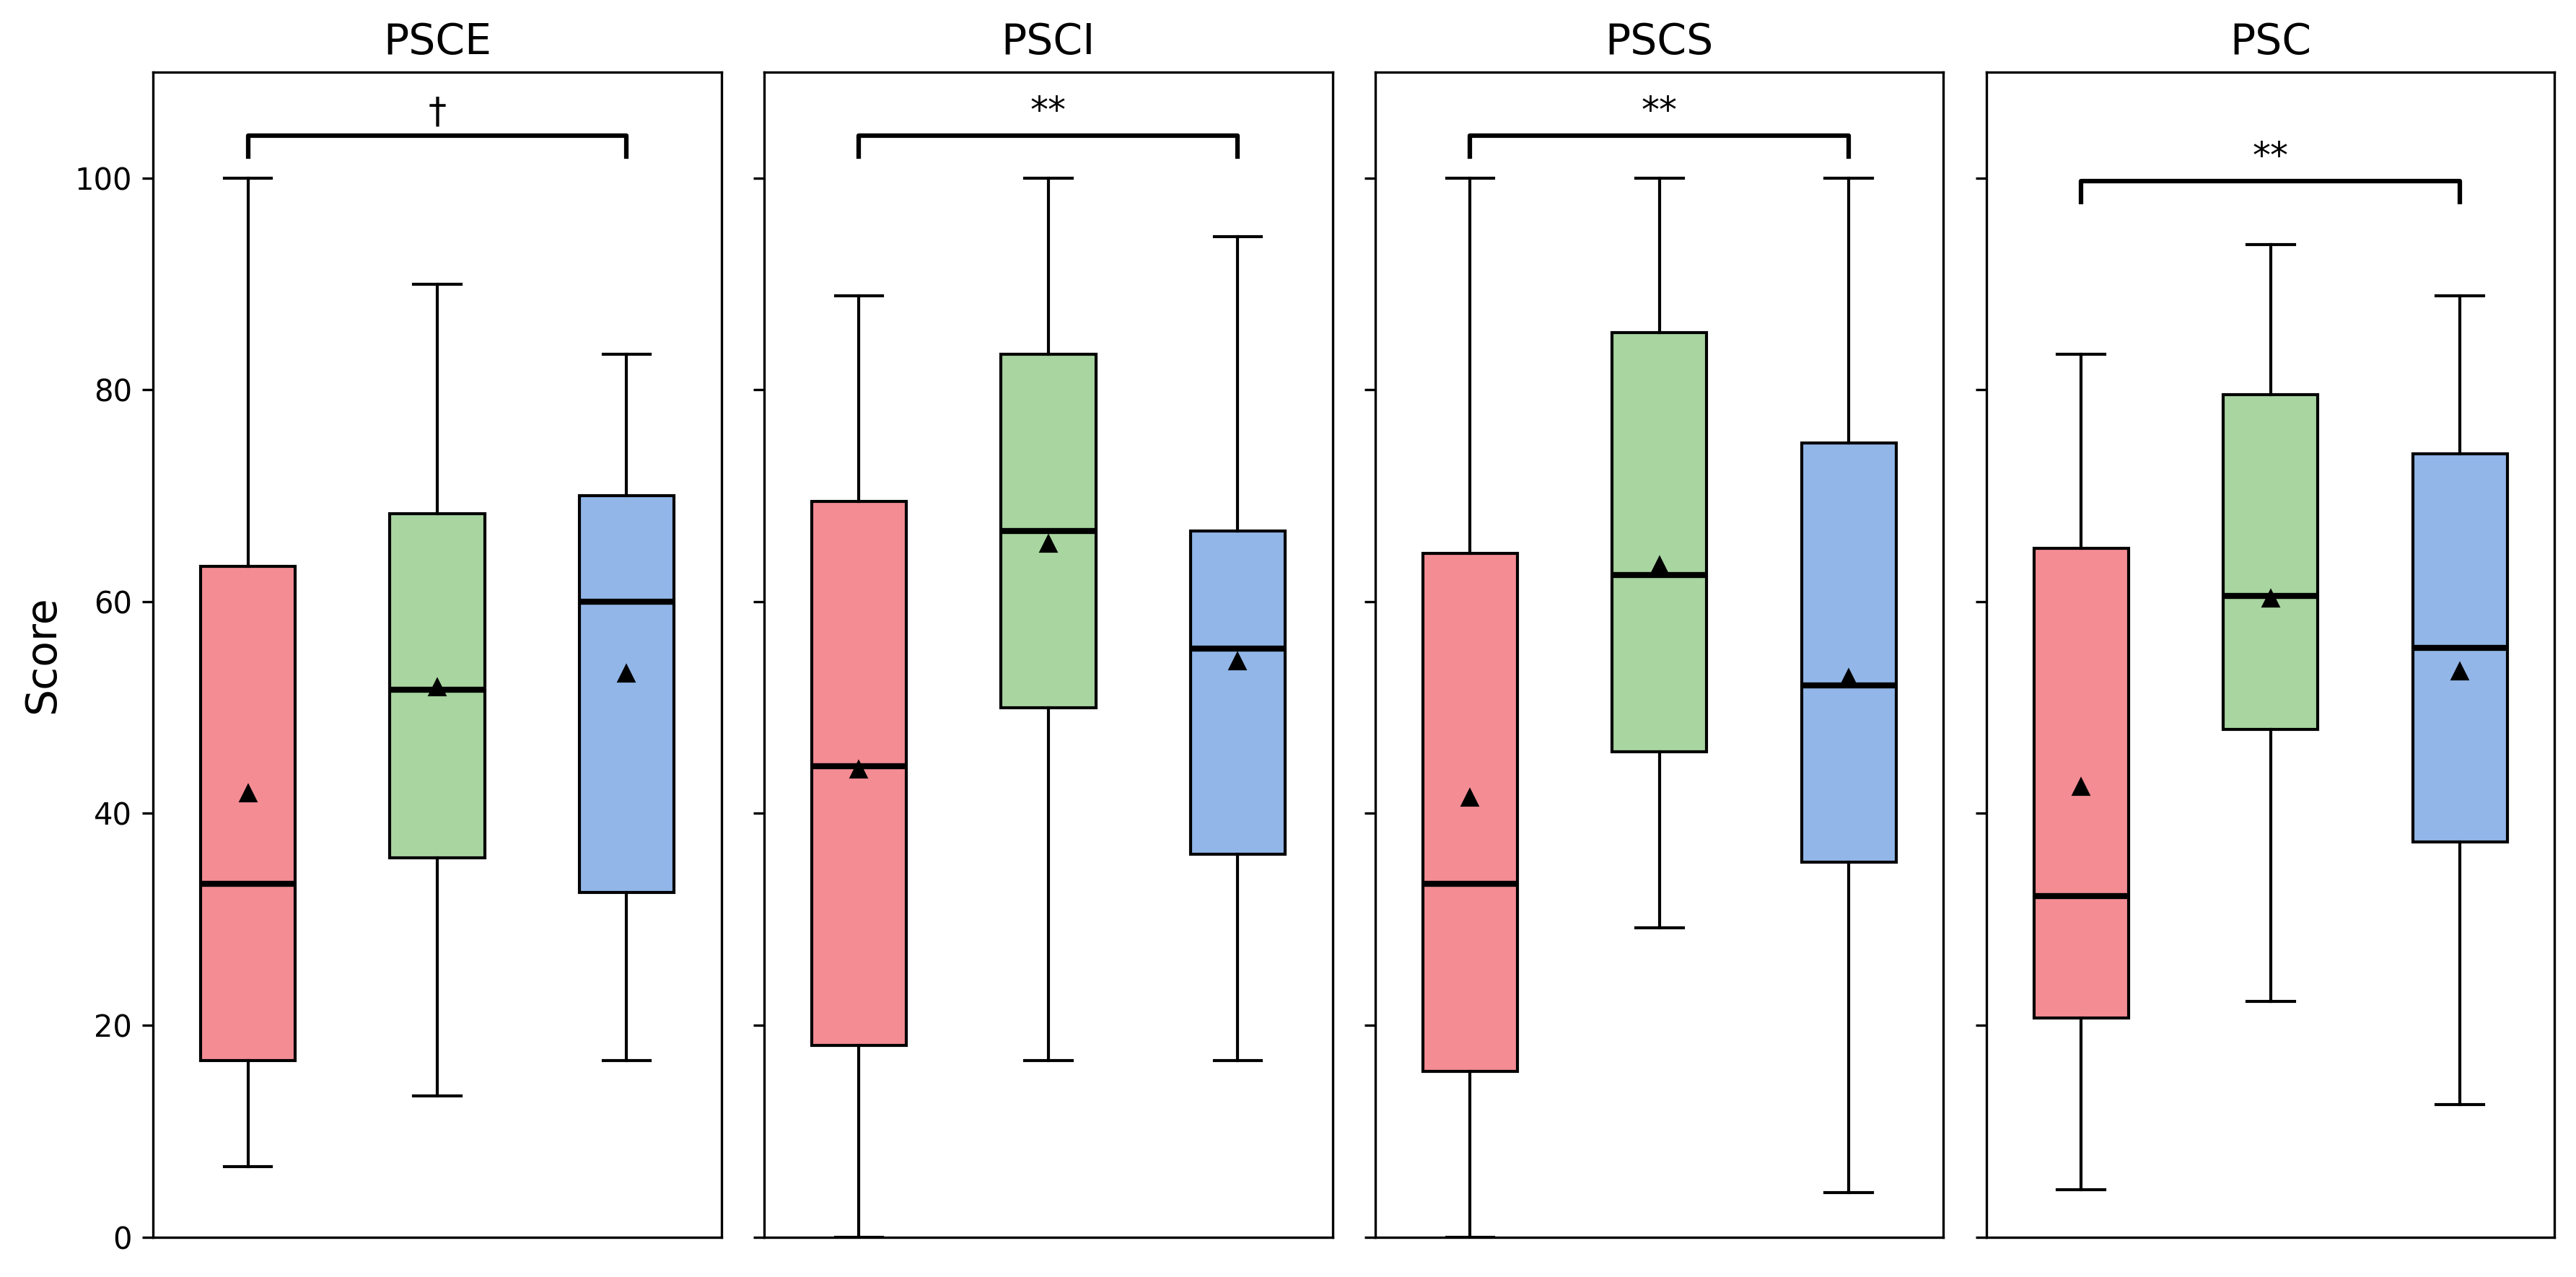
\includegraphics[height=4.7cm]{img/psc.png}
        \caption{PSC scales}
    \end{subfigure}
    \hfill
    \begin{subfigure}{0.12\linewidth}
        \centering
        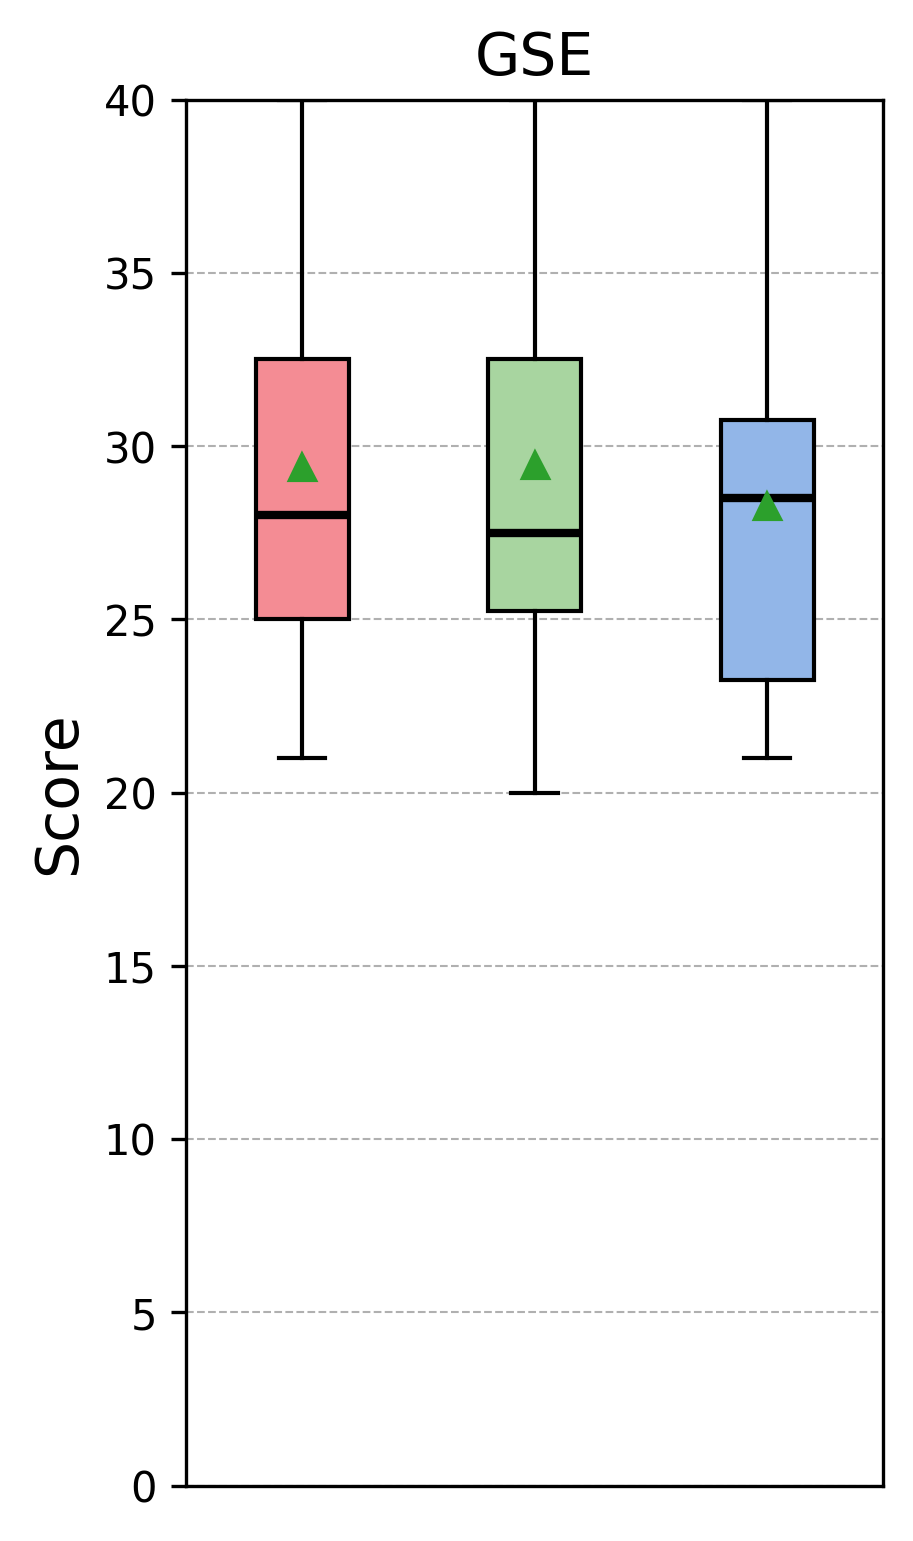
\includegraphics[height=4.7cm]{img/gse.png}
        \caption{GSE}
    \end{subfigure}
    \caption{Subjective measures across strategies: (a) overall workload (NASA-TLX), (b) perceived system curiosity (PSC subscales), and (c) general self-efficacy (GSE). S1 = Direct Querying, S2 = Parallel Exploration, and S3 = User-Preference-First}
\end{figure*}


\subsubsection{PSC}
We conducted normality tests on the scores of the Perceived System Curiosity (PSC) subscales. PSCE ($p = .009$) and PSCI ($p = .030$) deviated from normality, whereas PSCS ($p = .079$) and the overall PSC score ($p = .011$) satisfied the assumption of normality. Since several subscales violated normality assumptions, we employed repeated-measures ANOVA with Greenhouse--Geisser correction where appropriate. The results revealed significant effects of strategy on PSCI ($F(2,34) = 6.838, p < .01, \eta^2 = .29$), PSCS ($F(2,34) = 7.235, p < .01, \eta^2 = .30$), and the overall PSC score ($F(2,34) = 7.597, p < .01, \eta^2 = .31$). Expressive Curiosity (PSCE) only showed a marginal effect ($F(2,34) = 3.401, p = .063, \eta^2 = .17$). Pairwise comparisons further indicated that Strategy~2 yielded significantly higher scores than both Strategy~1 and Strategy~3 on PSCI, PSCS, and the overall PSC, while no significant differences were found between S1 and S3. 


\subsubsection{GSE}
For the General Self-Efficacy Scale (GSE), we first tested the normality of the overall scores. The results indicated a significant deviation from normality (Shapiro--Wilk, $W = 0.920, p = .002$). Since the homogeneity of variance assumption was satisfied (Levene’s test, $p = .973$), we conducted a Welch ANOVA to compare the three strategy conditions. The analysis showed no significant main effect of strategy on the overall GSE scores ($F(2,33.92) = 0.254, p = .777$, $\eta^2 \approx .009$). These findings suggest that the different strategies did not significantly influence participants’ general self-efficacy.


\subsection{Interview Results}

\textbf{Perceptual Differences Between Strategies}
When initiating the interviews, we asked all participants about the differences between the three strategies. \strategy{Parallel Exploration} was considered the most intelligent and efficient strategy by approximately 65\% of participants, capable of summarizing their preferences through a certain degree of interaction and effectively completing tasks. \smallitalic{"Parallel Exploration can infer my preferences based on my feedback, making it more efficient to organize."} \smallitalic{(P13)} In contrast, \strategy{Direct Querying} was perceived as mechanical by about 70\% of participants. \smallitalic{"Direct Querying asks for item locations one by one every time."} \smallitalic{(P08)} This was attributed to the strategy's repetitive questioning about item locations.
For \strategy{User-Preference-First}, approximately 60\% of participants perceived that this strategy inquired about user preferences at the beginning of the conversation and then categorized items based on those preferences.
\begin{quote}
\smallitalic{"User-Preference-First seems to ask general directional questions at first, and after finding a pattern, it starts asking about the relevance between pairs of items."} \smallitalic{(P17)}
\end{quote}

\textbf{Most Liked Strategy}
\strategy{Parallel Exploration} was the most popular strategy, chosen as the favorite by approximately 80\% of participants. The reason for this was its ability to efficiently summarize preferences and quickly provide personalized service:
\begin{quote}
\smallitalic{"Parallel Exploration allows me to complete the task in a shorter time because it can provide personalized recommendations based on my preferences."} \smallitalic{(P05)}
\end{quote}
Furthermore, one user considered its approach of summarizing patterns by arranging two or three items to be a positive performance: \smallitalic{"This strategy is very proactive, and its proactiveness is encouraging me."} \smallitalic{(P04)}
Approximately 15\% of participants chose \strategy{User-Preference-First} as their favorite strategy, primarily because it could summarize participants' preferences and make decisions based on them: \smallitalic{"User-Preference-First summarized my preferences. Although sometimes slower, it closely matches my needs."} \smallitalic{(P06)}
Although \strategy{Direct Querying} was less popular than \strategy{Parallel Exploration} and \strategy{User-Preference-First}, approximately 5\% of participants still considered it an effective strategy, especially for simpler tasks: \smallitalic{"Although Direct Querying is simple and direct, it is still effective when I only need simple categorization."} \smallitalic{(P12)}

\textbf{Least Liked Strategy}
\strategy{Direct Querying} was the most unpopular strategy, with about 70\% of participants considering it their least favorite. Its excessively high query frequency and lengthy interaction time led participants to generally perceive it as inefficient: \smallitalic{"Direct Querying requires me to answer each question individually. Although fast, it makes me feel repetitive and tedious."} \smallitalic{(P12)} The second least favorite was \strategy{User-Preference-First}. Although it could summarize preferences, the summarization process was slow: \smallitalic{"User-Preference-First although it can summarize my preferences, it takes a long time to process, often affecting my task progress."} \smallitalic{(P10)} Additionally, about 50\% of participants believed its summaries lacked accuracy, with one user even finding it aggressive: 
\begin{quote}
\smallitalic{"He is conscious and deliberately trying to explore my preferences, which makes me feel very aggressive."} \smallitalic{(P16)}
\end{quote}
For \strategy{Parallel Exploration}, only a small portion of participants found that: \smallitalic{"It sometimes gives incorrect classifications, which bothers me a bit."} \smallitalic{(P03)}

\textbf{Balancing Efficiency and Effectiveness}
\strategy{Parallel Exploration} was better at balancing effectiveness and efficiency, which was almost a consensus among most participants. \smallitalic{"Parallel Exploration not only provides personalized organization methods but is also more efficient and accurate in task execution."} \smallitalic{(P14)} In contrast, \strategy{Direct Querying} only asked about the placement of single items each time and did not group items according to participant preferences. It offered a more linear thought process that improved better outcomes: \smallitalic{"Direct Querying is good because it's very direct and clearly asks me where to put items."} \smallitalic{(P01)} However, its efficiency was low, making it the least efficient query method among the three strategies. \strategy{User-Preference-First} was pointed out by users for its low execution efficiency and inaccurate summarization process:
\begin{quote}
\smallitalic{"User-Preference-First can indeed summarize my preferences, but it is slow in processing and sometimes summarizes inaccurately, causing me to waste time."} \smallitalic{(P03)}
\end{quote}

\textbf{Teaching Confidence}
Most participants showed high confidence in \strategy{Parallel Exploration}, especially when it could summarize their preferences and execute tasks efficiently. P11 mentioned: \smallitalic{"Parallel Exploration can quickly summarize my preferences and complete tasks, so I have high confidence in it."} In contrast, confidence in \strategy{Direct Querying} and \strategy{User-Preference-First} was lower, particularly for \strategy{Direct Querying} which did not summarize participant preferences: \smallitalic{"Although Direct Querying is fast, I can't trust it because it doesn't summarize my preferences."} \smallitalic{(P18)}

\textbf{Interaction Burden}
Participants felt a heavier interaction burden with \strategy{Direct Querying} because the robot frequently asked for the placement of each item. Approximately 65\% of participants believed \strategy{Direct Querying} increased the cognitive load of the task, making participants feel troubled. P17 mentioned: \smallitalic{"Direct Querying requires me to answer every question each time, which is really stressful. Parallel Exploration makes it much easier for me."} \strategy{Parallel Exploration} and \strategy{User-Preference-First}, on the other hand, placed less pressure on participants in this regard because their query frequencies were significantly reduced, and they could even process items in batches based on their common attributes, further reducing the user's interaction burden.

\textbf{Situational Suitability}
In scenarios requiring explicit item order and position, \strategy{Direct Querying} might be more suitable as it clarifies the location of each item individually, avoiding confusion. This includes unfamiliar contexts, such as temporary accommodations, where personal preferences might not apply:
\begin{quote}
\smallitalic{"For example, going to a hotel by chance, or going for a picnic, or something like that. Then the placement of certain items may not follow the pattern of my long-term preferences. Such scenarios would be more suitable for Direct Querying."} \smallitalic{(P09)}
\end{quote}
It is also preferred in situations where high user control is needed to prevent unwanted robotic behavior:
\begin{quote}
\smallitalic{"Because I have a cat at home, and I'm afraid it might have some strange understanding and do something weird to the cat, causing my cat to get stressed. In such cases, I hope it constantly confirms every detail with me."} \smallitalic{(P04)}
\end{quote}

\textbf{Future Preference and Long-Term Use}
Users' expectations for future use are that the robot can learn their preferences within a short period and automatically summarize patterns when facing daily tasks, minimizing user disturbance as much as possible. Participants mentioned: \smallitalic{"I hope the robot can quickly adapt to my preferences in daily life. Parallel Exploration can do exactly that; it seems capable of meeting my long-term needs."} \smallitalic{(P14)} This indicates participants' advantages in adaptability and flexibility with \strategy{Parallel Exploration}. In contrast, \strategy{User-Preference-First}'s summarization is too slow, and when facing more complex daily scenarios, participants predict its response will be more sluggish. \strategy{Direct Querying} is too mechanical:
\begin{quote}
\smallitalic{"Especially since it needs to ask me the location of each item every time, it cannot self-adjust based on my preferences like Parallel Exploration."} \smallitalic{(P12)}
\end{quote}





\section{Discussion}
\subsection{User Perception and Differentiation of Strategies}
Our findings indicate that users were able to clearly perceive differences between questioning strategies and form consistent judgments about them. The questionnaire results revealed significant contrasts across conditions: Parallel Exploration was perceived as more “curious,” Direct Querying as mechanical and burdensome, and User-Preference-First as offering some value in inferring preferences but at the cost of efficiency. These outcomes were corroborated by NASA-TLX, where Direct Querying reduced interactional complexity but was associated with redundancy and frustration, while Parallel Exploration increased perceived intelligence and proactivity but also raised cognitive demand. 

Interviews further illuminated these perceptual mechanisms. Most participants described Parallel Exploration as the most intelligent and efficient strategy because it could infer their preferences with limited exchanges, echoing earlier work that links perceived competence with positive robot evaluations~\cite{bartneck2009measurement}. In contrast, Direct Querying was often characterized as “repetitive” and “mechanical,” lacking flexibility—an observation consistent with findings that overly rigid interaction patterns undermine user engagement~\cite{naneva2020systematic}. User-Preference-First was valued for helping establish a categorization framework, but its inaccuracy and slower pace often hindered task progress. Such differences not only reflect strategic variation but also how users construct mental models of the robot: some framed it as a “tool” or “butler,” prioritizing efficiency and execution, while others treated it as a “friend” or even a “child,” expressing patience and willingness to “teach” it over time, in line with prior research on anthropomorphism and role attribution~\cite{de2016almost}. 

Taken together, these findings suggest that participants were able to go beyond noticing surface differences and instead formed distinct interpretations of the three strategies. Parallel Exploration was often understood as a proactive way of inferring preferences, Direct Querying as a rigid and repetitive approach, and User-Preference-First as cooperative but slow. Within our tasks, these distinctions shaped how participants reasoned about the robot’s role and capability, influencing whether they framed it as efficient, mechanical, or in need of guidance.



\subsection{Task and Individual Modulators}
Our study further shows that task characteristics substantially shaped strategy preferences. Familiar tasks led participants to favor direct and minimal questioning to avoid redundancy, whereas unfamiliar or ambiguous situations made exploratory strategies more acceptable. Task frequency and importance also influenced expectations of strategy switching. For everyday chores such as tidying a desk, participants preferred robots to gradually learn general rules and reduce interruptions, while for important tasks such as organizing documents they welcomed step-by-step confirmation for accuracy and control. These observations resonate with prior work showing that user expectations for household robots vary by task familiarity and criticality~\cite{yoo_2024_preferences,bansal_2020_supportive}. They also extend evidence that goal-oriented tasks with well-defined outcomes (e.g., placing a single item) often favor preference-first questioning, while process-oriented tasks requiring multiple interdependent steps (e.g., packing a suitcase) invite ongoing exploration~\cite{hu2025task}. 

Individual traits played an equally critical role. Dominant users emphasized efficiency and control, thus preferring direct strategies. Participants with established organizational rules resisted over-exploration, while others without strong rules appreciated additional probing. Parallel exploration proved particularly divisive: some perceived it as intrusive or “aggressive,” reflecting broader concerns about privacy and boundaries in HRI~\cite{cucciniello2023mind}, whereas others described the robot as “child-like” and expressed patience in teaching it, consistent with findings that anthropomorphism can foster tolerance and trust~\cite{de2016almost}. Such polarized responses explain why our questionnaires did not always reveal significant differences, while interviews exposed more nuanced patterns. 

Finally, participants emphasized the challenges of multi-member households, where different users may hold conflicting expectations—one favoring efficiency and directness, another appreciating exploratory engagement. This highlights the need for personalized memory and multi-user modeling to balance competing demands, in line with emerging research on adaptive and multi-user HRI~\cite{rosenthal2010mixed}. Taken together, these findings suggest that task properties and individual differences jointly modulate strategy preferences, reinforcing the importance of adaptive, user-centered questioning frameworks. 

\subsection{Efficiency, Experience, and Long-Term Trade-offs}
We observed a tension between efficiency and experience. Direct Querying kept workload low but felt repetitive due to item-by-item prompts, whereas Parallel Exploration appeared more intelligent and proactive yet raised cognitive demand as it probed for richer information. These patterns support a conservative querying policy: the system should ask only when the expected value of information outweighs the interruption cost, a classic mixed-initiative principle that aligns with active preference-learning approaches designed to minimize queries while learning user objectives~\cite{biyik2019asking}.

Participants also emphasized that short-term impressions do not capture long-term needs. They wanted the robot to remember household rules, avoid redundant questions in routine contexts, and re-query only when uncertainty genuinely increases. Prior work on long-term HRI highlights the role of gradual personalization and memory in sustaining engagement~\cite{matheus2025long}, and recent results in domestic tidying show that compact preference summaries can generalize across related scenarios~\cite{wu2023tidybot}. Taken together, within our tasks this points to memory-augmented, context-aware strategy switching as a practical path to maintain comfort over time.


\subsection{Bridging the HHI–HRI Gap}
 The gap between human–human (HHI) and human–robot (HRI) questioning is especially salient in domestic contexts. In HHI, people naturally mix explicit questions with subtle cues—pointing, gaze, or shared routines—so that preference elicitation rarely feels repetitive. Robots, by contrast, rely on a narrow communication channel: limited prosody, rigid timing, and a lack of nonverbal signals make even simple questions sound mechanical, particularly during everyday tasks like tidying where efficiency is valued~\cite{mutlu2009footing}. Latency further disrupts the flow of collaboration, leading users to perceive interruptions as unnecessary effort.
 
Memory and uncertainty also create friction. In households, humans build up shared context over time (e.g., where items “usually” belong or which rules are exceptions). Current systems, however, often fail to retain preferences across sessions or to judge when re-asking is worthwhile~\cite{leite2013social,ji2023survey}. As a result, the same strategy that feels exploratory in HHI can feel redundant or inefficient in HRI. Users tolerate one-time clarification but become frustrated when a robot repeatedly asks about obvious or previously answered choices~\cite{ahn2022can}.

To close this gap, questioning strategies must adapt to the domestic setting: improving interaction bandwidth with socially legible cues, while also incorporating memory-augmented, cost-aware policies that minimize repetitive queries and leverage past household knowledge. In this way, robots could elicit preferences when uncertainty is high but otherwise act autonomously, allowing strategies that work in HHI to feel more natural in long-term, everyday HRI.

\subsection{Limitations}
Questioning strategies may change over the course of long-term, life-long interactions. Our short-term controlled study cannot capture how preferences and robot behaviors evolve when interactions extend over weeks or months. Understanding these dynamics will be essential for assessing sustainable impacts on user experience and robot learning. 

The current implementation tested strategies in isolation. For experimental control, human questioning patterns were abstracted into single strategies, but in reality people often mix or switch strategies dynamically. This simplification improves interpretability but reduces ecological validity. Future work should explore how robots can flexibly adjust or combine strategies in real time, balancing efficiency, personalization, and user comfort. 

Evaluation was limited to a single household task. While this ensured comparability across participants, it constrains generalizability. Real-world household environments involve diverse and evolving tasks, where robust performance requires both task-specific adaptation and the ability to generalize across contexts. Future studies should investigate whether the identified strategies support such generalization and transfer. 


\section{Conclusion}
This work examined how robots can learn household tasks by asking questions. We first identified three distinct questioning patterns in a formative human-human study—Direct Querying, Parallel Exploration, and User-Preference-First—confirming that people naturally employ different ways of eliciting information (RQ1). We then implemented these patterns as controllable strategies in a VLM-based framework and demonstrated their consistent deployment in multi-turn interaction (RQ2). A user study ($N=18$) showed that the strategies led to significant differences in efficiency, sense of control, workload, and task outcomes (RQ3). Together, these findings show that questioning strategies can be systematically studied and compared as part of robot learning by asking, and that human-derived patterns can be concretely instantiated as controllable robot behaviors in real household tasks.
%%
%% The next two lines define the bibliography style to be used, and
%% the bibliography file.
\bibliographystyle{ACM-Reference-Format}
\bibliography{sample-base}


%%
%% If your work has an appendix, this is the place to put it.
\appendix

\section{K-type Categories}
\begin{table}[htbp]
\centering
\caption{K-type category \cite{10.1145/3568294.3580077}}
\label{tab:k-type}
\begin{tabular}{lll}
\hline
\# & Categories     & Description \\
\hline
K1  & Identity         & Information about who or what a person or thing is \\
K2  & Class            & Inclusion relationships of categories \\
K3  & Attributes       & Properties or features of the object \\
K4  & Quantities       & Quantitative specifications \\
K5  & Spatial layout   & Spatial relations among entities \\
K6  & Temporal relation& Temporal information or sequences \\
K7  & Contents         & Additional detailed information \\
K8  & Procedure        & Order or method of a specific process \\
K9  & Causality        & Causal chains of events or states \\
K10 & Intention        & Motivation, aim or plan of another agent \\
K11 & Internal state   & Mental states such as preference or mood of another agent \\
\hline
\end{tabular}
\end{table}



\section{Task Materials and Layouts}
\label{app:items}

Figure~\ref{fig:layouts} shows the initial setups of the three tidying tasks. Each setup included 10--12 items distributed across a central table and 2--3 designated storage areas. The object composition and spatial layout were carefully designed to be comparable in complexity while still allowing for individual variation in preferences (e.g., categorization, accessibility, or arrangement).  

\begin{figure}[t]
    \centering
    \includegraphics[width=\linewidth]{img/layout_1.png}
    \caption{Initial layouts for the three household tidying tasks: bar counter(left), study desk (middle), and office desk(right). Each scenario contains approximately 10--12 items and 2--3 storage spaces, designed with comparable complexity while preserving room for individual preferences.}
    \label{fig:layouts}
\end{figure}


\subsection{Item Lists}
\label{app:items}

\begin{table}[h]
\centering
\begin{tabular}{ll}
\toprule
\textbf{Item} & \textbf{Attributes} \\
\midrule
Plate & Black, with white bird pattern \\
Bowl & Small, white, with gold rim \\
Brush & Gray sponge brush on a stick \\
Sauce & Glass jar with red cap \\
Noodles & Instant noodle cup, red and black \\
Detergent & Bottle of yellow dish soap \\
Oil & Glass bottle of cooking oil \\
Spoon & White, ceramic \\
Sponge & Yellow, wavy shape \\
Sponge & Yellow, wavy shape \\
Lemon & Yellow, whole fruit \\
\bottomrule
\end{tabular}
\caption{Bar counter tidying item list.}
\end{table}

\begin{table}[h]
\centering
\begin{tabular}{ll}
\toprule
\textbf{Item} & \textbf{Attributes} \\
\midrule
Bottle & Transparent, plastic, with green cap \\
Notebook & Cork cover \\
Book & White, pink and green cover \\
Book & White cover, ``Design as Art'' \\
Fan & White, round \\
Measure & Retractable tape measure \\
Tape & Roll of black electrical tape \\
Sunglasses & Brown lenses, black frame \\
Keyboard & Black, Logitech brand \\
Basket & Silver, wire mesh \\
Bin & Blue, plastic \\
Doll & Gray, owl-shaped doll \\
\bottomrule
\end{tabular}
\caption{Office desk tidying item list.}
\end{table}


\begin{table}[h]
\centering
\begin{tabular}{ll}
\toprule
\textbf{Item} & \textbf{Attributes} \\
\midrule
Lamp & White, phone holder style \\
Mouthwash & Transparent bottle with blue \\
Toolset & Orange and transparent \\
Yogurt & White, plastic bottle \\
Baseball & White with red stitching \\
Doll & Brown, bear-shaped doll \\
Tissues & Blue and white package \\
Thermos & Light green \\
Gamecard & Green Xbox game case \\
Gamecard & Black GTA game case \\
Umbrella & Black and white striped \\
Remote & White, air conditioner remote \\
\bottomrule
\end{tabular}
\caption{Study desk tidying item list.}
\end{table}

\end{document}
\endinput
%%
%% End of file `sample-sigconf-authordraft.tex'.
